\documentclass[12pt]{article}
\usepackage{listings}
\usepackage[utf8]{inputenc}
\usepackage{xcolor}
\usepackage{gensymb}
\usepackage{amsmath}
\definecolor{codegreen}{rgb}{0,0.6,0}
\definecolor{codegray}{rgb}{0.5,0.5,0.5}
\definecolor{codepurple}{rgb}{0.58,0,0.82}
\definecolor{backcolour}{rgb}{0.95,0.95,0.92}
\definecolor{color0}{rgb}{0.2,0.2,0.2}
\definecolor{color1}{rgb}{1, 0, 0}
\definecolor{color2}{rgb}{1, 0.5, 0.5}
\definecolor{color3}{rgb}{0.9,0.9,0.9}
\definecolor{color4}{rgb}{0,0.1,0.9}
\definecolor{color5}{rgb}{0.1,0.9,0.1}
\definecolor{color6}{rgb}{0.5,0.2,0.08}
\definecolor{color7}{rgb}{1, 0.271, 0}
\definecolor{color8}{rgb}{0.502, 0, 0.502}

\lstdefinestyle{mystyle}{
    float=tp,
    floatplacement=tbp,
    backgroundcolor=\color{backcolour},   
    commentstyle=\color{codegreen},
    keywordstyle=\color{magenta},
    numberstyle=\tiny\color{codegray},
    stringstyle=\color{codepurple},
    basicstyle=\ttfamily\footnotesize,
    breakatwhitespace=false,         
    breaklines=true,                 
    captionpos=b,                    
    keepspaces=true,                 
    numbers=left,                    
    numbersep=5pt,                  
    showspaces=false,                
    showstringspaces=false,
    showtabs=false,                  
    tabsize=2
}

\lstset{style=mystyle}
\usepackage{graphicx} % Required for inserting images
\usepackage[style=ieee]{biblatex}
\addbibresource{ref.bib}
\usepackage[letterpaper]{geometry}
% \usepackage[letterpaper, total={6in, in}]{geometry}
\renewcommand*{\bibfont}{\footnotesize}

\begin{document}
\title{3D2Mol: Converting Molecular Model Images to Digital Representations to Improve Student Understanding}


\author{Wenqi Marshall Guo\\
Department of CMPS\\
University of British Columbia\\
Kelowna, BC\\
wg25r@student.ubc.ca 
\and
Mohamed Shehata\\
Department of CMPS\\
University of British Columbia\\
Kelowna, BC\\
mohamed.sami.shehata@ubc.ca
}

\maketitle


\begin{abstract}
Concrete molecular models could be important tools for students to learn organic chemistry compared to the virtual models. However, it lacks some properties of virtual models such as being able to look up more information (e.g. boiling point, polarity, name, etc) about the molecule. Thus, we aim to close the gap between concrete models with their digital representations. In this paper, we built a computer rendered and a real-world dataset of molecular models.We than trained a deep learning model on the datasets that can convert an image of real-world molecular models into simplified molecular-input line-entry system (SMILES). We tested beam search, multi-image input, and self-reflection to increase the accuracy of the model. 

\end{abstract}


\section{Introduction}
Molecular models are helpful tools in chemistry education as they provide an intuitive way for students to understand the 3D structure compared to 2D molecular structure representation. These models can also assist students with 3D mental operations. 
% Although virtual models could be as effective as concrete models, concrete should be available to students at least at the beginning of the study of new concepts and ideas, as humans sometimes rely on concrete objects.\autocite{savec_evaluating_2005} 
A study \autocite{savec_evaluating_2005} found that although virtual models could have the same effectiveness as concrete models, students should have access to concrete models at least at the beginning of the study because sometimes humans rely on concrete objects. Additionally, digital model tools have a learning curve, and it is hard for students to understand some space operations such as a ``chair flip" or bonds rotation using digital models. 
However, digital model representation has the benefit that allowing students to look up more information about the molecule such as the IUPAC (International Union of Pure and Applied Chemistry) name, the boiling point, and the polarity. Students can also modify the molecule and observe how it will affect the molecular properties. Thus, it will be beneficial if students can convert concrete molecular models to digital representations. 


Although there are models that can convert 2D molecular structure representations to corresponding digital representations \autocite{swinocsr}\autocite{decimer}\autocite{chempix}, to the best of our knowledge, there is not a model for 3D molecular models. It will be beneficial to chemical education to close this gap between 3D molecular models and digital representations. 
Our contribution to this paper can be summarised as:
\begin{itemize}
\item We have constructed two datasets: one computer-rendered 3D molecular model and another consisting of real-world 3D molecular models.
\item We trained a model on top of these two datasets that is capable of converting images of concrete molecular models into their respective SMILES (simplified molecular-input line-entry system) notations. 
\item We applied a method based on multi-image input and beam search to increase the accuracy of the output.
\item  We proposed to let the model re-evaluate its output and select the one with the highest probability of being correct.
% can we use this for seg? review the segmented images
% \item We applied a multi-image input method allowing users to capture multiple images of the molecular model to increase the accuracy of the output.
\end{itemize}

\section{Related Work}
To the best of our knowledge, there is no prior model that can convert a 3D molecular set photo into its digital structure representation. However, there are some models for 2D structure formulas. The two most recent ones are SwinOCSR\autocite{swinocsr} and DECIMER.ai\footnote{The name DECIMER has been used by the same team for both the dataset and two versions of the mode, here we are refreshing the model published in 2023.}\autocite{decimer}. These two models are very similar in architecture consisting of an image encoder and a transformer. The architecture of DECIMER.ai and SwinOCSR are shown in Figure \ref{fig:rwa}.
ChemPix is another model that attempted to recognize hand-drawn hydrocarbon structures using CNN and Long Short-Term Memory (LSTM).  

\begin{figure}
    \centering
    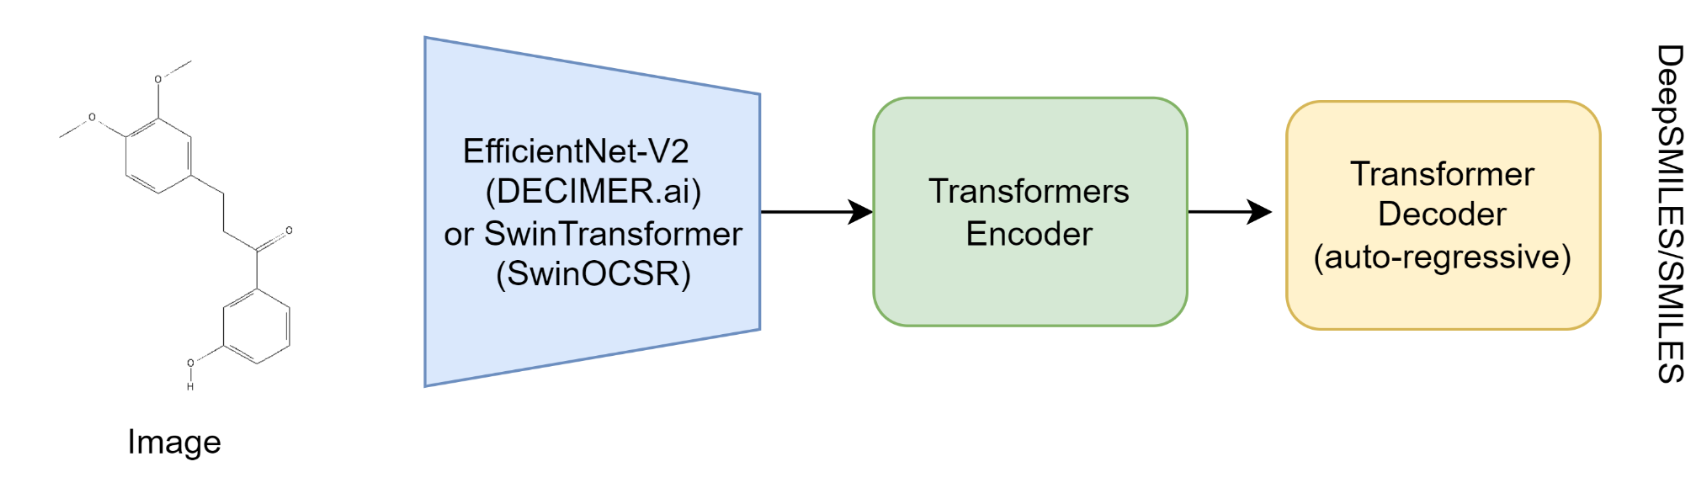
\includegraphics[width=\textwidth]{related_work_arch.png}
    \caption{Model Architecture of DECIMER.ai and SwinOCSR}
    \label{fig:rwa}
\end{figure}
% The decoder used in 
\subsection{DECIMER.ai}
In DECIMER.ai, the encoder is an EfficientNet-V2-M. EfficientNet is a type of convolutional neural network (CNN) with MBConv \autocite{tan_efficientnet:_2020} (a modified version of the inverted bottleneck from \autocite{mobilenet}) and Fused-MBConv \autocite{suyog_efficientnet-edgetpu:_2019} developed by training-aware neural architecture search (NAS). \autocite{swin_tran} \autocite{effv2} MBConvs have 1$\times$1 point-wise and 3$\times$3 depth-wise convolutional layers, which can yield better parameters and computational efficiency. \autocite{mobilenet} \autocite{effv2} However, they cannot fully utilize modern hardware accelerators. In Efficient-Net-V2, they proposed using regular 3x3 convolutional layers (Fused-MBConvs) to replace MBConvs for the early stages of the network. This results in better training time with small overheads of parameters and FLOPs. In an MBConv block used in Efficient-Net-V2, the image is first passed through a 1x1 convolutional layer to increase its channel numbers, then a squeeze and excitation (SE) block is used \autocite{hu_squeeze-and-excitation_2019}\autocite{tan_efficientnet:_2020}. SE blocks are shown to increase the performance of CNNs with slight computational overhead. \autocite{hu_squeeze-and-excitation_2019}. The SE block is followed by a depthwise 3x3 convolution and a 1x1 convolution, the latter decreases the channel counts to the same as input. In a Fused-MBConv, however, the depthwise convolution and the 1x1 convolution are replaced by a 3x3 convolution. \autocite{effv2} \autocite{mobilenet}

The decoder in DECIMER.ai is a transformer model based on \autocite{attention_is_all_you_need}. It has four transformer encoder blocks and four transformer decoder blocks with right parallel attention heads. \autocite{decimer} The encoder of the transformer utilizes a multi-head self-attention block and an MLP (multilayer perceptron) to replace previous recurrent neural or convolutional layers. The decoder of the Transformer is auto-regressive, meaning the decoder of the model takes in the already generated sequence and predicts the next token. The generated sequence will be processed by a masked multi-head self-attention. The mask will prevent the model from attending tokens after $t$ when generating the $t$-th sequence. Then a cross-attention layer is applied that connects the input sequence and the generated sequence by using the output of the encoder as keys and values and output from the masked self-attention as the query. Then the output of the cross-attention is followed by an MLP layer. The encoder and decoder blocks are repeated for $N$ (In DECIMER.ai $N=4$) times each. After the last decoder block, the output goes through a linear and a softmax layer before output. Since attention does not consider position information, position encoding is added to the sequence for both input and generated sequences. The full transformer also uses residual connection across all the attention and MLP layers. After the addition of the residual connection, a layer normalization is used. A detailed architecture of the Transformer can be found in the original paper \autocite{attention_is_all_you_need}. 

Although DeepSMILES \autocite{oboyle_deepsmiles:_2018} has been proposed for machine learning models to generate more valid identifies, their previous work \autocite{rajan_performance_2022} has shown that SMILES actually lead to the most accurate identifiers, SELFIES \autocite{krenn_self-referencing_2020} generated the most valid sequences, and SMILES is between the two. Thus, they used SMILES instead of DeepSMILES in DECIMER.ai. \autocite{decimer}  

DECIMER.ai is trained on 127.5 million molecules (453.9 million depictions) with image size of 512$\times$512. They tested the model on the in-domain dataset with 250K images each. The testing set does not contain molecules from the training set. The results show DECIMER.ai can generate molecules with Tanimoto similarity greater than 0.95 and average sequence-level accuracy greater than 75\%. The detailed performance result could be found in their original paper \autocite{decimer}. 

In addition to printed structure formulas, which have regular shapes and format, DECIMER.ai also attempted to recognize hand-drawn structures by finetuning the model with a dataset that has augmented data that makes structures look hand-drawn. This increases sequence level accuracy from 27\% to 60\% and increases the Tanimoto similarity from 0.2 to 0.89.
\autocite{decimer} 

%how it trained on real data and handwritten 
\subsection{SwinOCSR}
In SwinOCSR, the encoder (they referred to as ``backbone" in their paper) is built on the Swin Transformer. The image is cut into patches with each path having a size of $4 \times 4$ pixels. Then each patch is flattened into and treated as a token which is a 48-dim vector. Then a linear projection layer is applied and each token is into a 192-dim space. 
Then 4 Swin-Transformer (Shifted Window Transformer) \autocite{swin_tran} blocks are used. Each swim transformer block contains two regular transformer modules. In the first transformer module, Window Mutli-head Self Attention (W-MSA) is performed within each window, which is a group of neighbouring tokens. In the second transformer module, the Shifted Window Mutli-head Self Attention (SW-MSA) is performed on a shift-ed window. The W-MSA allows the model to capture the local relationship in the image, and the SW-MSA introduced a cross-window connection while maintaining efficiency. Before the tensor ($H_i \times W_i \times C_i$) gets passed to the next Swin Transformer block, a patch merging operation is performed to capture hierarchical information. During path merging, neighbouring $2 \times 2$ patches are merged and the tokens are concatenated. This results in $\frac{1}{4}$ of the number of patches and each $4C_i$ feature for each token. Then the dimensions of each token are reduced to $2C_i$. In SwinOCSR, 4 Swin Transformer blocks are used; the last Swin Transformer block outputs a tensor with shape $\frac{H}{32} \times \frac{H}{32} \times 1536$. This tensor is flattened across the spatial axes and projects the last axis into 256 dimensions. 
% After each block, a patch merging operation is performed such that neighbouring patches are merged and the tokens are contacted. \autocite{swin_tran} The decoder of SwinOCSR is very similar to the decoder in DECIMER.ai, which is also a transformer encoder-decoder pair but with 6 blocks of encoders and 6 blocks of decoders. 
In addition, SwinOCSR uses focal loss \autocite{lin_focal_2018} instead of normal cross-entropy loss due to the imbalance of the tokens distribution. \cite{swinocsr} Original focal loss is only for binary task and \autocite{swinocsr} rewrited it for muti-class, which is shown in Equation \ref{focal} and \ref{focal2}, where $\sigma$ is the sigmoid function, $O_i$ is the output logist from the network, and $p_i$ is the probility of each class. 
\begin{equation}
    p_i = \begin{cases} \sigma(o_i) &  y_i=1 \\
    1-\sigma(o_i) & \text{otherwise} \\
    \end{cases}
    \label{focal}
\end{equation}

\begin{equation}
    L = \frac{1}{n}\sum_i^n -a_i(1-p_i)^\gamma log(p_i)
\end{equation}

% Moved down here To this point, we get a tensor of $\frac{H}{4} \times \frac{W}{4} \times 48$ where $W$ and $H$ are the width and height of the original image. 
% Before the tensor ($H_i \times W_i \times C_i$) gets passed to the next Swin Transformer block, a patch merging operation is performed to capture hierarchical information. During path merging, neighbouring $2 \times 2$ patches are merged and the tokens are concatenated. This results in $\frac{1}{4}$ of the number of patches and each $4C_i$ feature for each token. Then the dimensions of each token are reduced to $2C_i$. In SwinOCSR, 4 Swin Transformer blocks are used; the last Swin Transformer block outputs a tensor with shape $\frac{H}{32} \times \frac{H}{32} \times 1536$. This tensor is flattened across the spatial axes and projects the last axis into 256 dimensions. 

%how it trained using a special loss function  
% deepsmiles


% \subsection{Re-evoluate the Results After Generation}
\subsection{ChemPix}
ChemPix \cite{chempix} is a model aimed at recognizing hand-drawn hydrocarbon (molecules with only carbon and hydrogen atoms, showing in structure formulas as mostly lines without letter notations) structures to their SMILES strings. They use a network architecture adapted from image captioning, with a CNN as the encoder and an LSTM with an attention mechanism and beam search as the decoder. \cite{chempix} They limited their dataset with ring size less than 8 carbons and molecules with multiple conjoined rings are not considered. They use both synthetic and real hand-drawn images to train the model. They also used a ``voting committee" consisting of multiple models to vote for the final answer.

% \subsection{Math Formula to LaTeX Conversion}
% Besides OCSR, another simlar 

\subsection{Perfomance Comparsion}
In DECIMER.ai \autocite{decimer}, they compared the performance between DECIMER.ai and other OCSR software, including SwinOCSR. They tested the sequence-level accuracy and Tanimoto similarity on a series of datasets. To test the robustness of the models, they added distortions (i.e. rotating for $\pm5\degree$ and shearing) to all datasets. The comparison of DECIMER.ai and SwinOCSR is shown in table \ref{compare}. \autocite{decimer} For detailed information, such as the data distribution and for performances of other models, please refer to the DECIMER.ai paper \autocite{decimer}. They concluded that DECIMER.ai achieves competitive results and its performance did not get negatively affected by distortion in the data. SwinOCSR did not achieve outstanding results in this benchmark; the developer of SwinOCSR observed that their model dose does not perform well on real-world data, possibly due to a lack of diversity in the training data. \autocite{decimer} \autocite{swinocsr} 

\begin{table}[]
    \centering
    \begin{tabular}{c|c|c|c|c|}
      &  \multicolumn{2}{c|}{Undistorted Dataset} & \multicolumn{2}{c|}{Distorted Dataset} \\ \hline
      & DECIMER.ai & SwinOCSR & DECIMER.ai & SwinOCSR \\ \hline
     Sequence-Level Accuracy & \textbf{65\%} & 14\% & \textbf{68 \%}  & 8\%\\
     Tanimoto & \textbf{93\%} & 70\% & \textbf{96 \%} & 64\%\\
     Proportion of Tanimoto=0 & \textbf{2\%} & 5\% & \textbf{1\%} & 8\%\\
     Proportion of Tanimoto<0.3 & \textbf{3\%} & 9\% & \textbf{2\%} &16\%\\

    \end{tabular}
    \caption{Perfomance Comparison Between DECIMER.ai and SwinOCSR}
    \label{compare}
\end{table}
\section{Method}
We also used a two-stage training process in our project, similar to \autocite{decimer} and \autocite{chempix}. The model is first trained on a synthetic (3D rendered) dataset and then finetuned on a real-world collected dataset to reduce the amount of real-world data that needs to be collected as they are expensive.  


\begin{figure}[t]
    \centering
    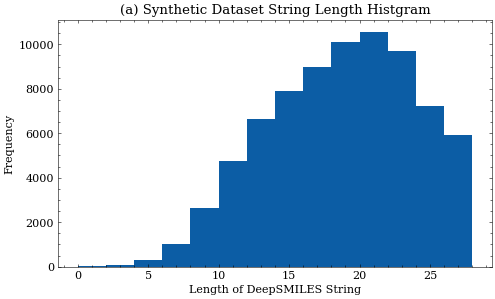
\includegraphics[width=0.45\textwidth]{sy_len.png}
    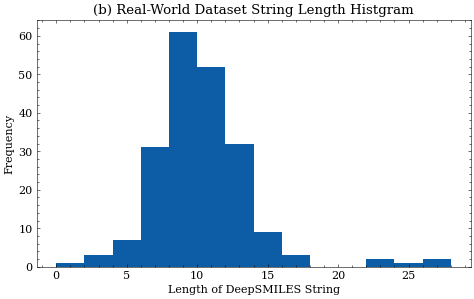
\includegraphics[width=0.45\textwidth]{real_len.png}
    \caption{DeepSMILES String Length Distributions}
    \label{fig:dis}
\end{figure}

\subsection{Synthetic Dataset}
\begin{figure}[t]
    \centering
    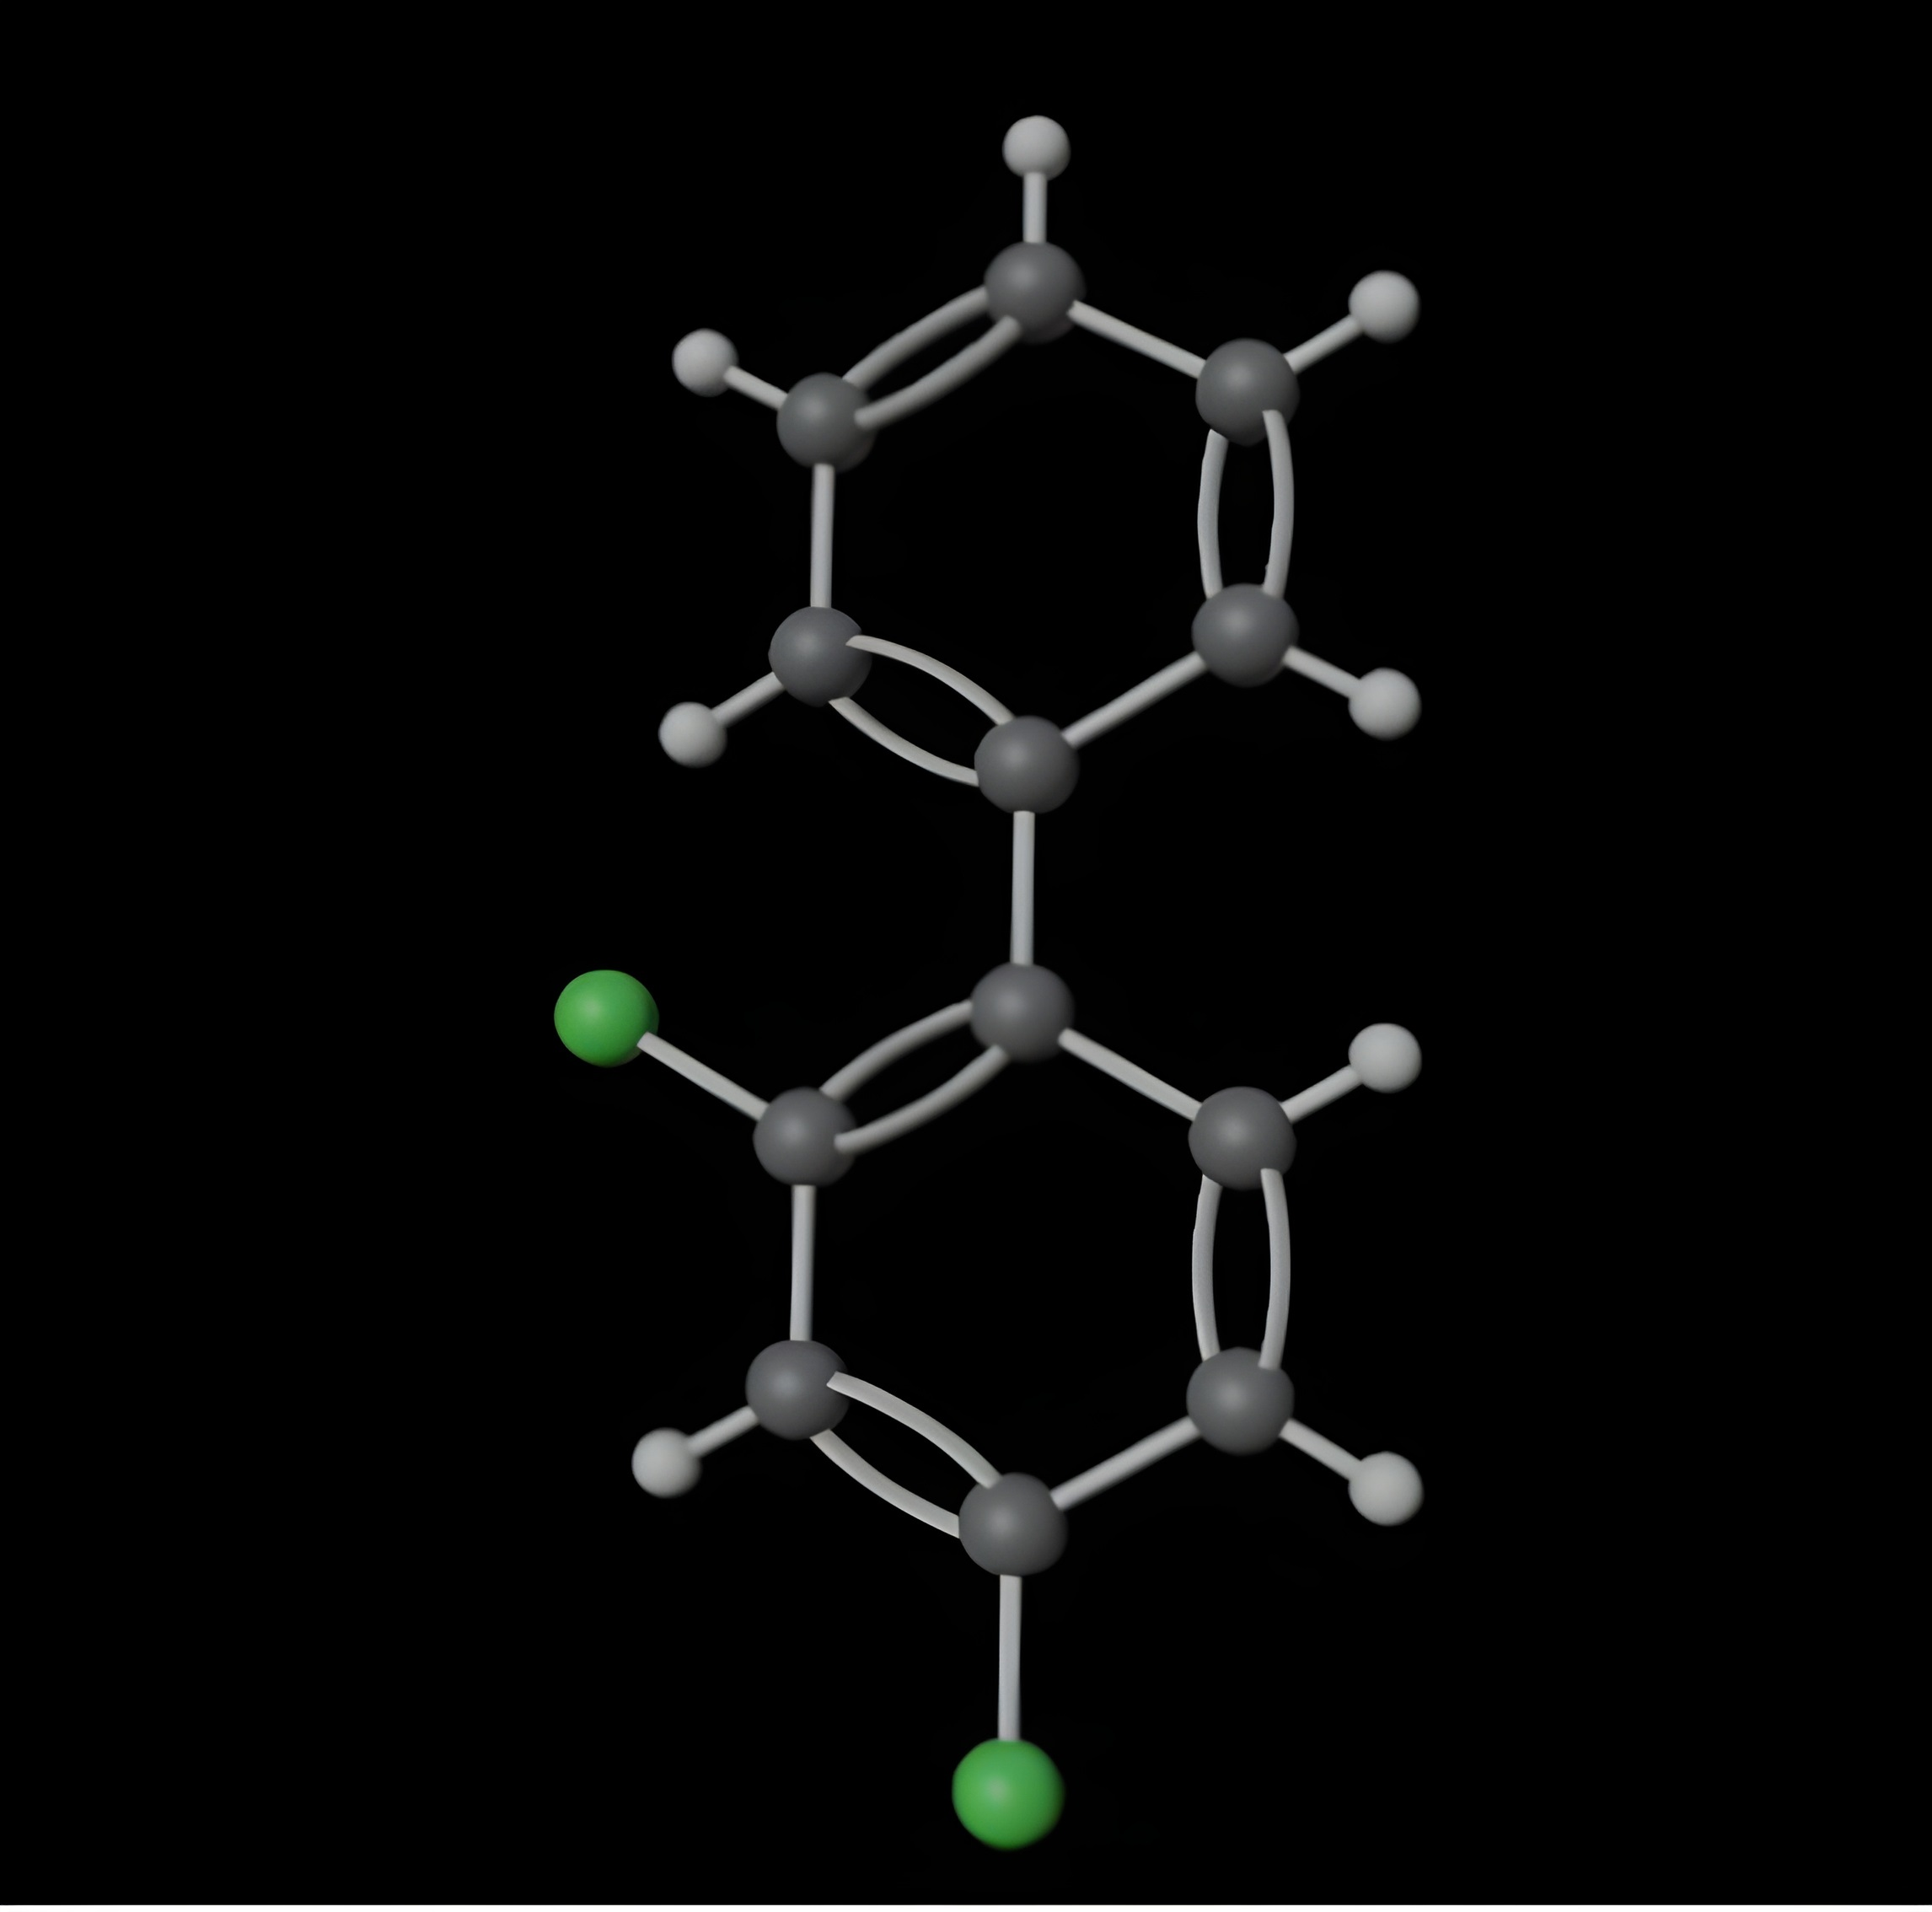
\includegraphics[width=0.3\textwidth]{generated}
    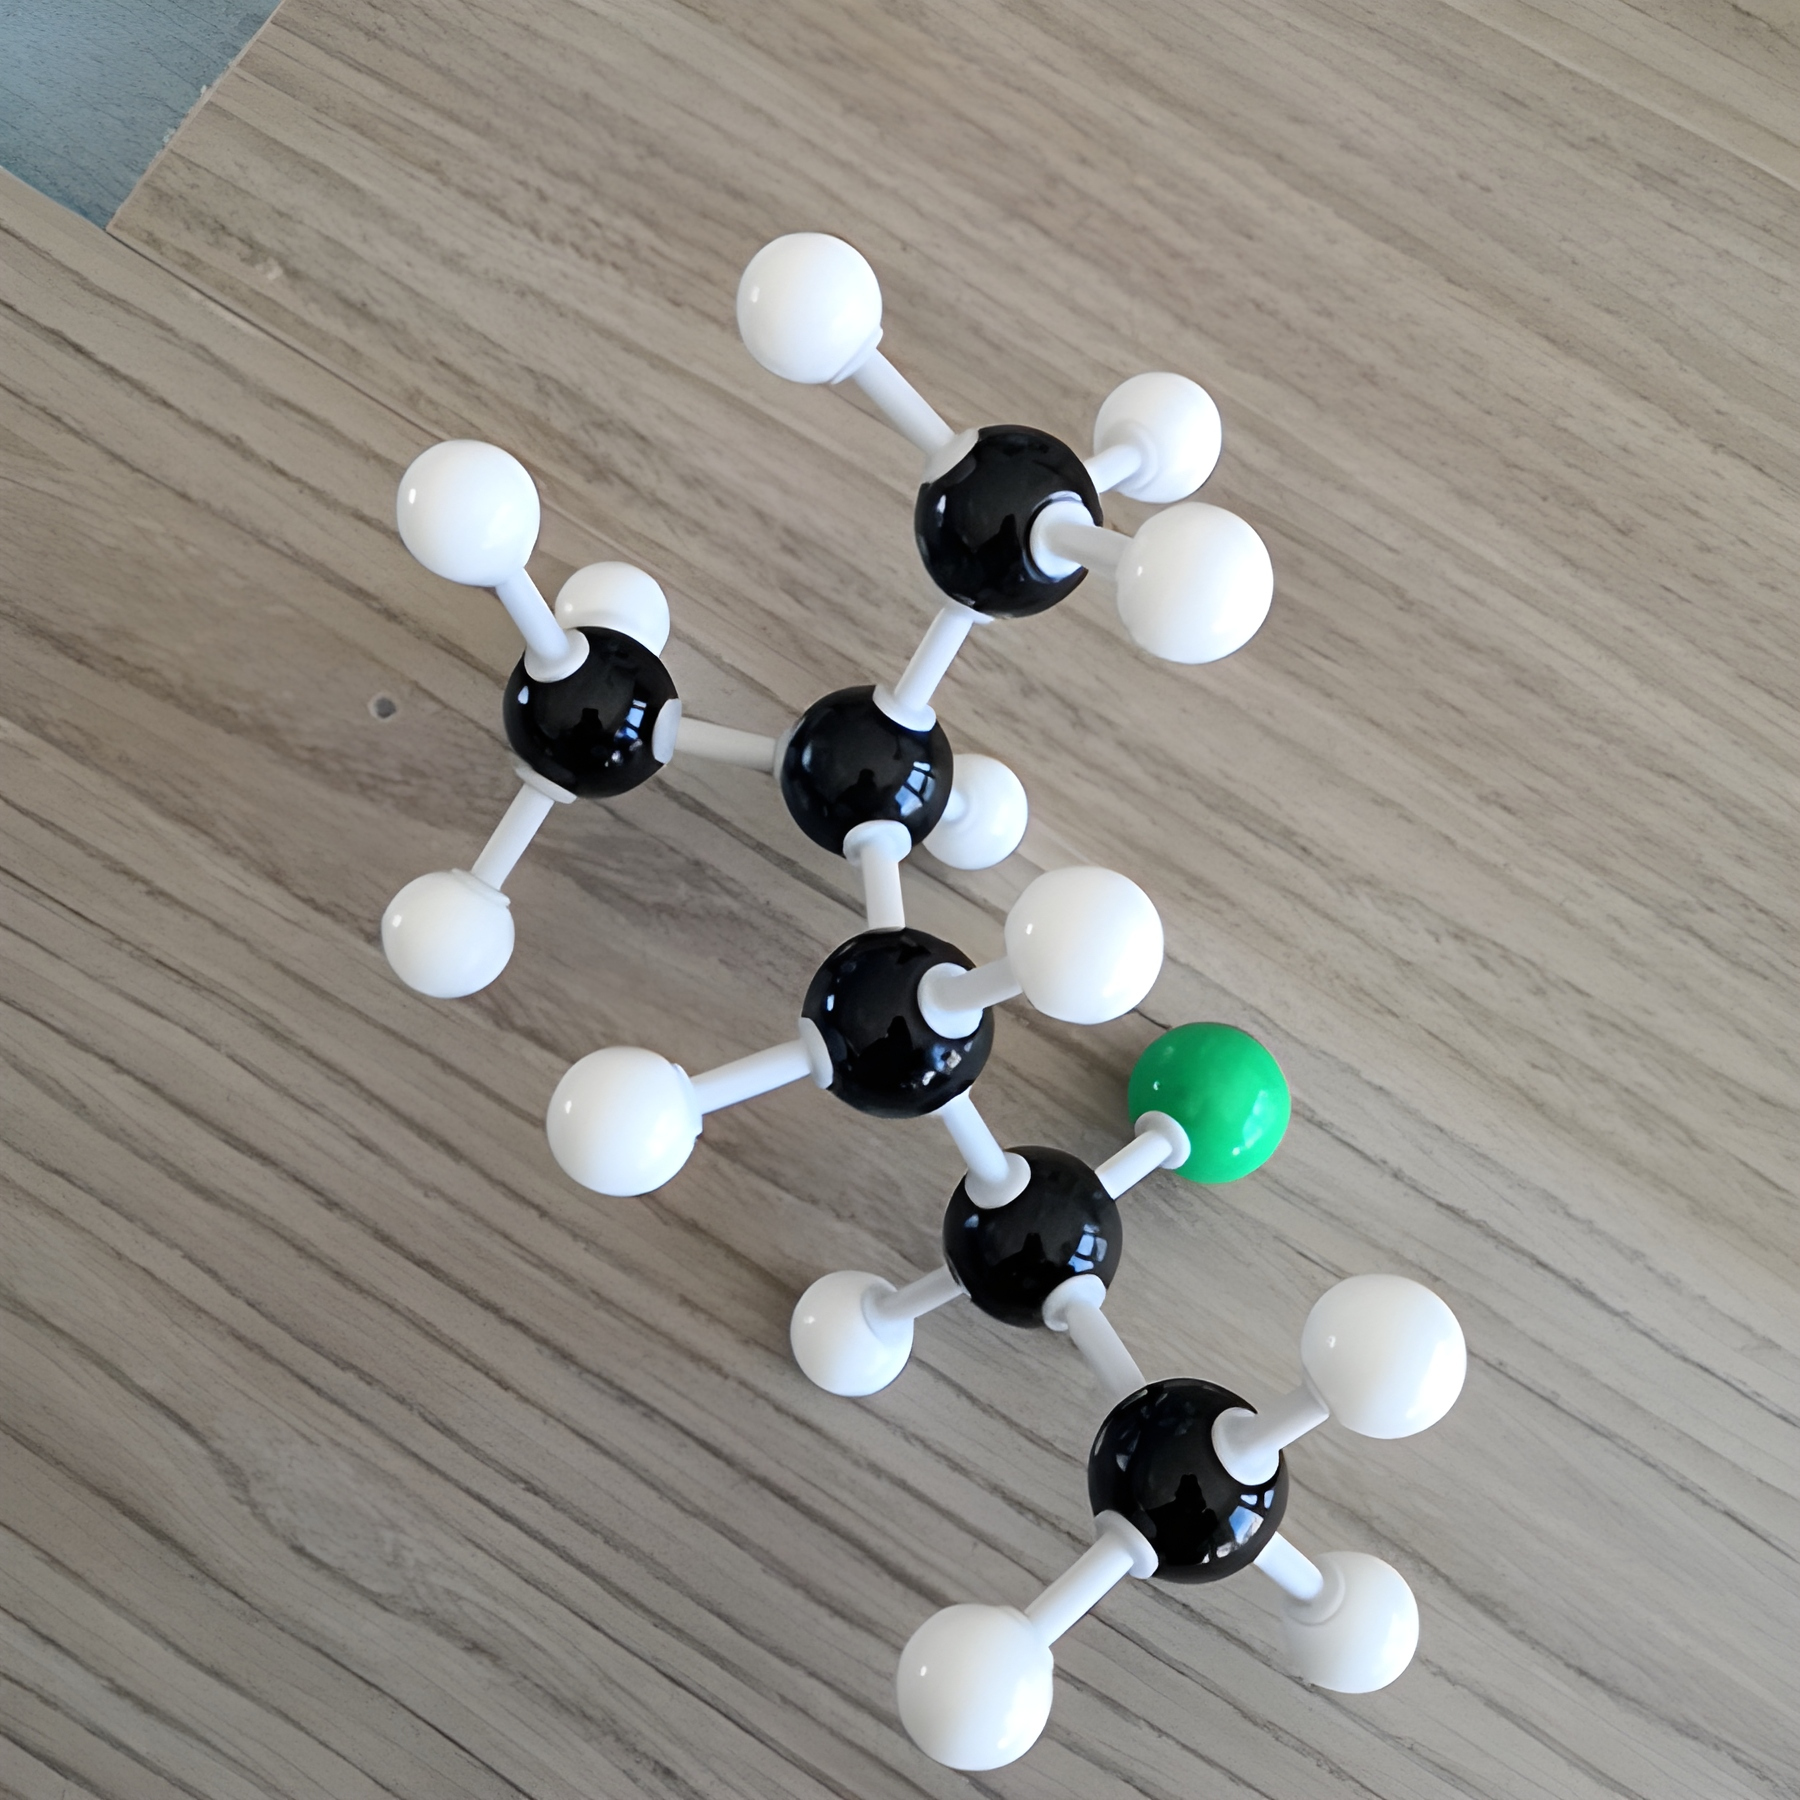
\includegraphics[width=0.3\textwidth]{cap}
    \caption{A rendered image and a real captured image of 2-Chloro-4-methylpentane}
    \label{fig:example}
\end{figure}

We downloaded a set of compounds from PubChem \autocite{kim_pubchem_2023}, and then these compounds were filtered based on heavy atoms and molecular weights and only contained elements of C, O, S, H, N, Cl, Br, F, and P. Because of the complex 3D nature of molecules, there could be occlusions between atoms and bonds, where important information is hidden in the image. Although there are methods to avoid occlusions by some spatial algorithm or human selection, we decided to remove 3D spatial information in the pretraining stage. Thus, we downloaded the 2D coordinate from PubChem instead of 3D.  
% filtered such that the compounds have at most X atoms \footnote{We did not directly limit the number of atoms on PubChem queries: we limited the number of heavy atoms and molecular weight, which yielded in the limitation of atoms.} 
After filtering, there are 79,369 compounds in the dataset. We created a Blender Python Script to render these compounds into 3D molecular images. OpenAI ChatGPT was used to write the building blocks (API Wrapper) and some logic of the script. The colour of each atom follows the CPK colouring convention (shown in Table \ref{cpk}) and was according to a couple of online sources and 3D molecular models on the market. The atoms are rendered using spheres, single bonds are rendered using cylinders, and double bonds are rendered using torus. For each molecule, we rendered 4 different images at different angles. Detailed render process can be found in our GitHub repository. 
% self negative example: gan
% Rendered from 2D information ....
\begin{table}[]
    \centering
    \begin{tabular}{c|c|c}
        Element & Color & RGBA Code \\ \hline
C & \textcolor{color0}{\textbf{*}} & (0.2,0.2,0.2,1)\\
S & \textcolor{color2}{\textbf{*}} & (1, 0.5, 0.5, 1)\\
H & \textcolor{color3}{\textbf{*}} & (0.9,0.9,0.9, 1)\\
N & \textcolor{color4}{\textbf{*}} & (0,0.1,0.9, 1)\\
Cl &  \textcolor{color5}{\textbf{*}} & (0.1,0.9,0.1, 1)\\
Br & \textcolor{color6}{\textbf{*}} & (0.5,0.2,0.08,1)\\
F & \textcolor{color7}{\textbf{*}} & (1, 0.271, 0, 1)\\
P & \textcolor{color8}{\textbf{*}} & (0.502, 0, 0.502, 1)\\
    \end{tabular}
    \caption{CPK Coloring Convention Used in Rendering}
    \label{cpk}
\end{table}
%redo
We observed that image size will affect the convergence speed of the model and the traditional image size used for classification ($224\times224$) is not enough for our task; thus, we used an image size of $400\times400$. 
\subsection{Real-World Dataset}
We created a mobile application using React.js for data collection. The application will show the user a 3D interactive model pre-view by \autocite{rego_3dmoljs_2015} and allow the user to capture multiple images of the model they built. The application screenshot can be found in the Appendix. To increase the efficiency of data collection, we group similar models using the GPT: a list of the names of the molecules is given to the GPT via the OpenAI API and asked to group similar molecules together. Users can build either the given molecules or another molecule they choose. Volunteers are recruited to collect these images of molecular models. Because some of the molecular model kits we used do not have sulphur, we excluded all molecules with sulphur. After collecting, we observed some low-quality data such as images with obstruction between atoms, motion blur, etc. Thus, we made another application allowing volunteers to go through all the images and decide if they would be kept or discarded. The images are collected on clear backgrounds, and for each molecule images with different camera angles are captured. In total, we have a total of 1934 images of 203 molecules. 

We separated the training set and validation set by SMILES strings (i.e. different images of the same molecule will not appear in both validation and training set. Since we ignored isotopes here, molecules with different IDs might have the same SMILES) The validation set is randomly selected such that it has 20 molecules and 214 images total. 

\begin{figure}[t]
    \centering
    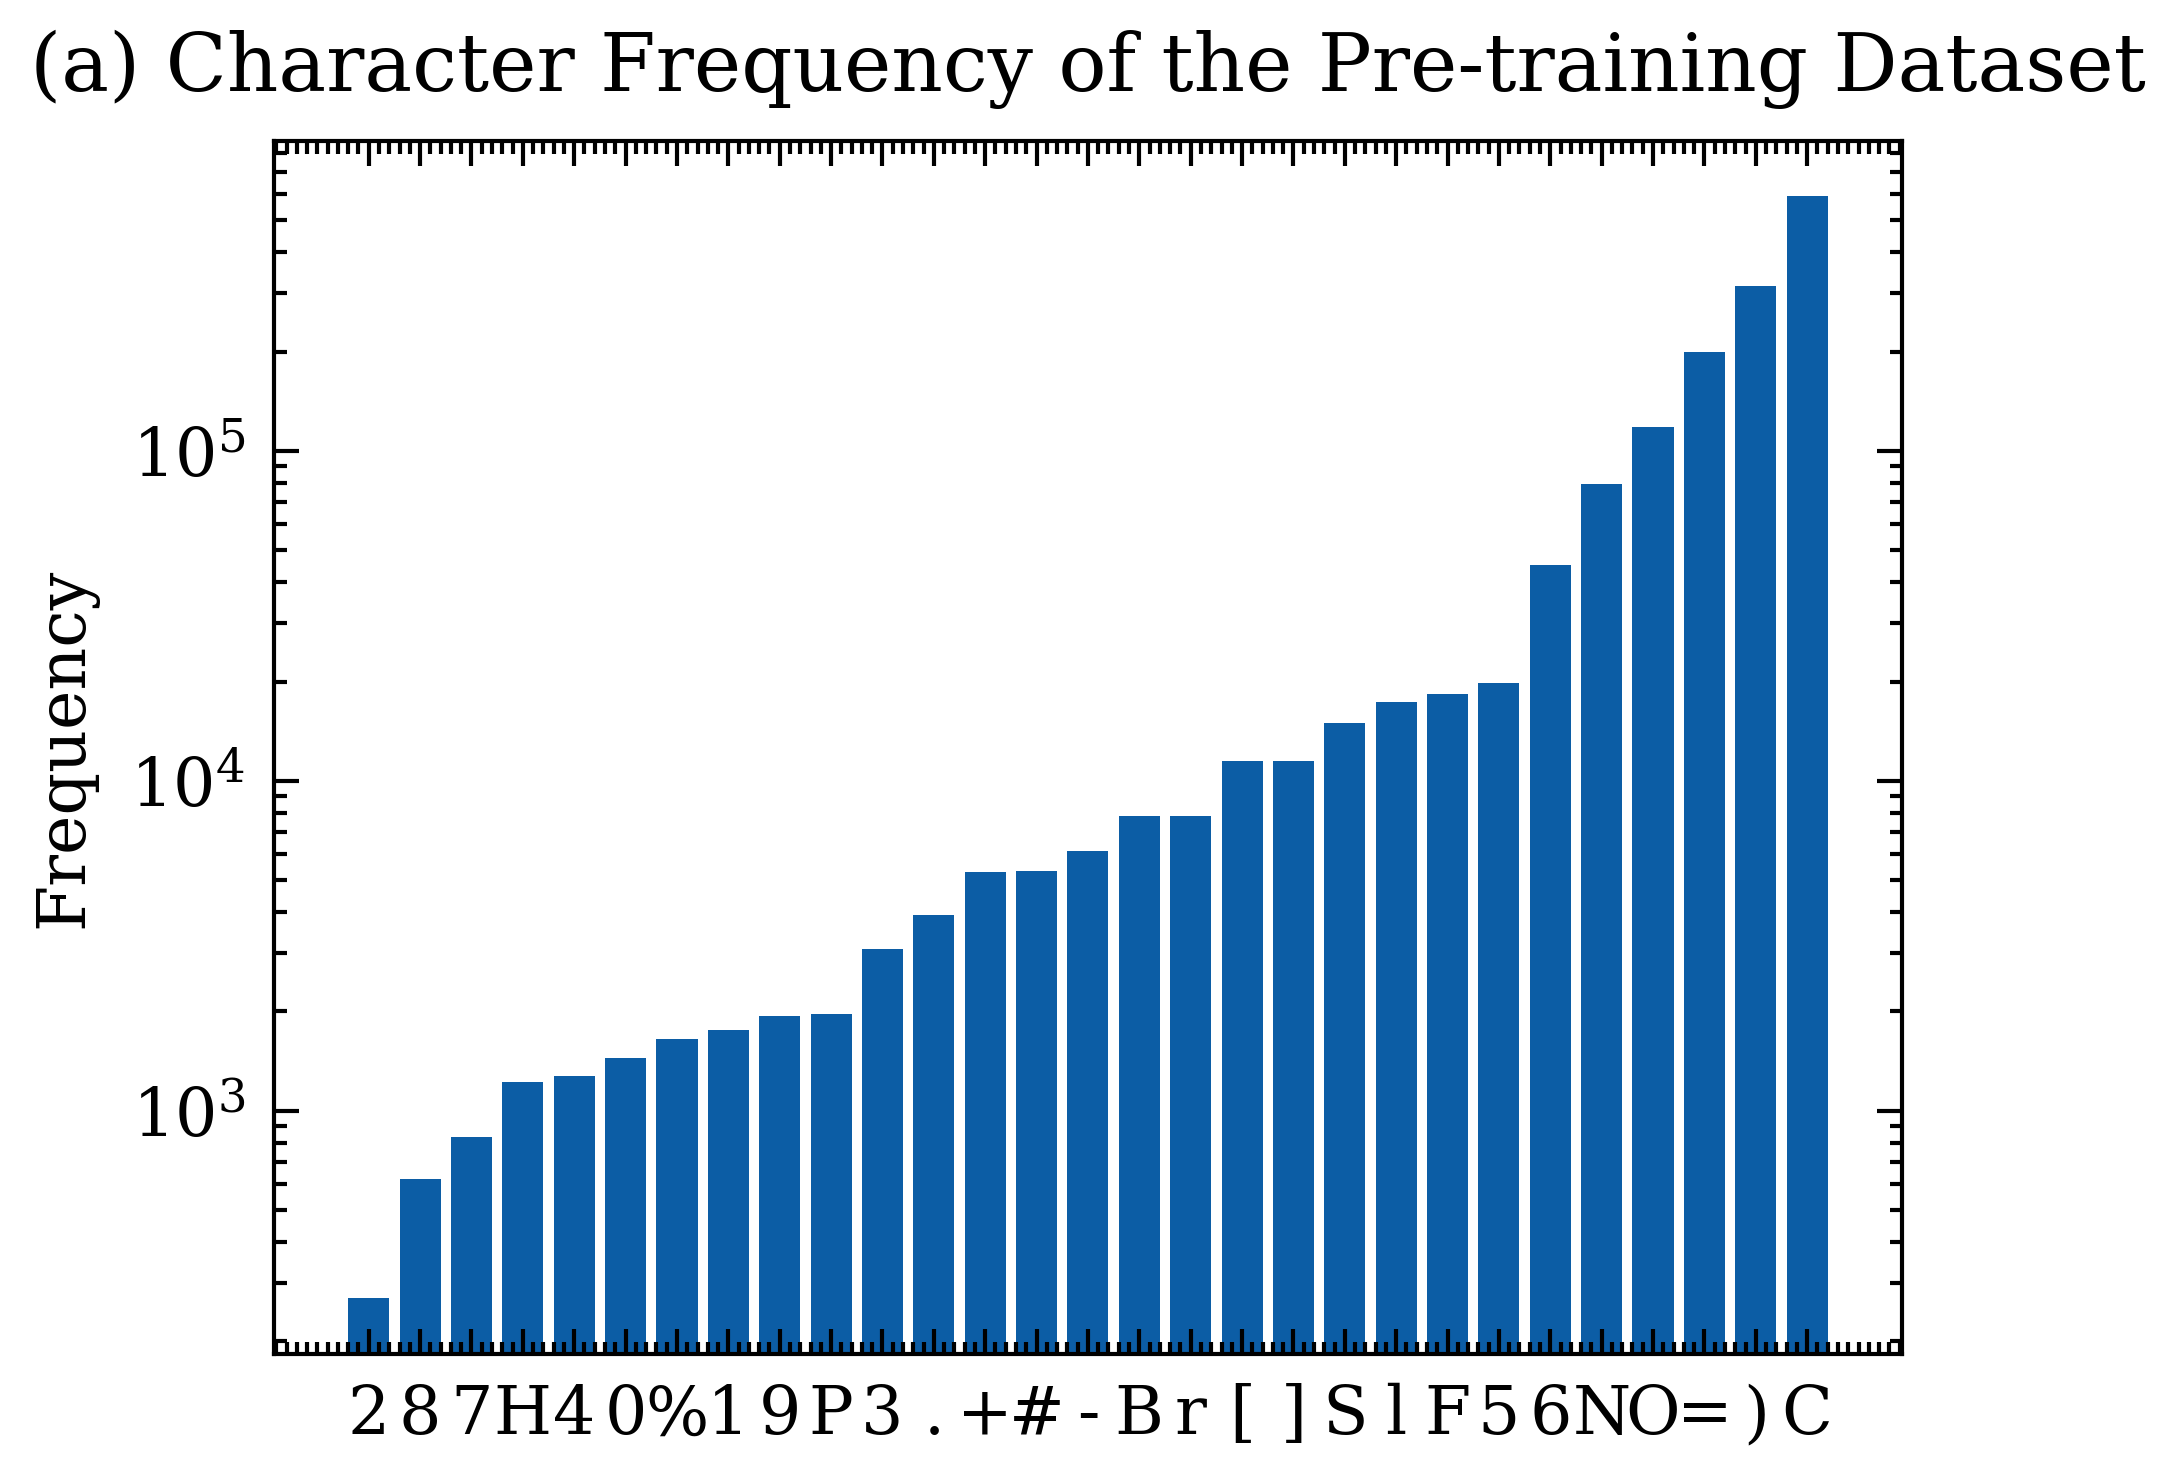
\includegraphics[width=0.4\linewidth]{freq1.png}
    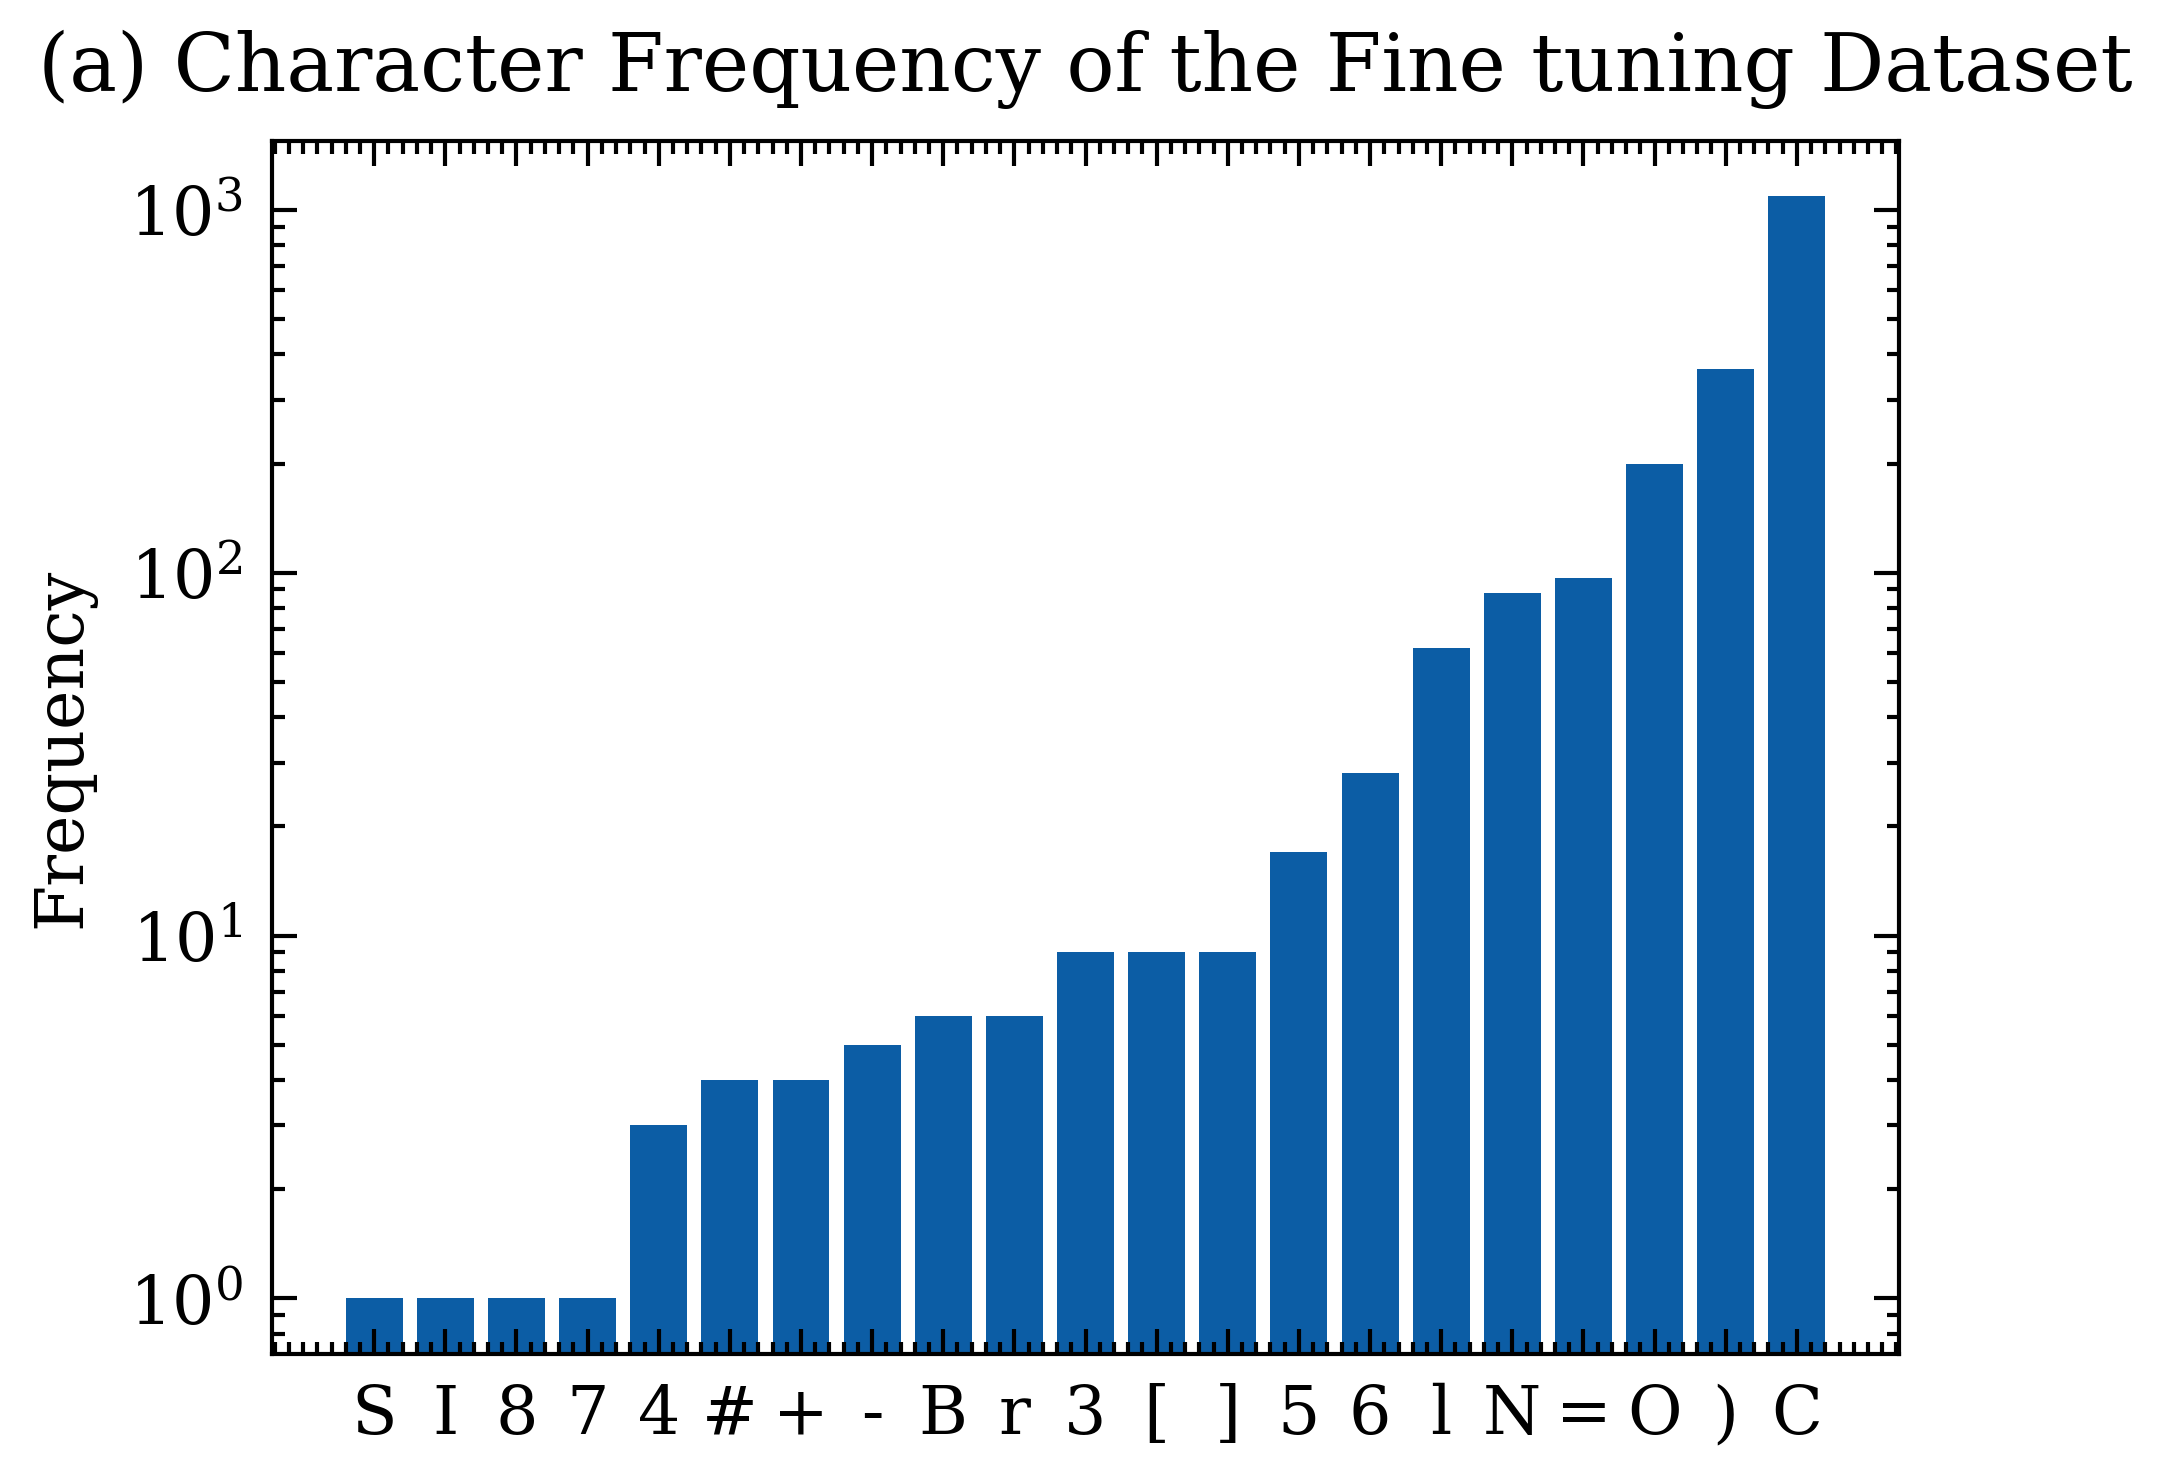
\includegraphics[width=0.4\linewidth]{freq2.png}
    \caption{Character Frequency Distribution}
    \label{chardis}
\end{figure}
Figure \ref{fig:example} shows an example of rendered and real images. These images are images from the dataset after super-resolution for better visualization. Figure \ref{fig:dis} shows the DeepSILES string length distribution and Figure \ref{chardis} shows the character frequency distribution of both datasets. 


\subsection{Machine Learning Model} 
\subsubsection{Basic Model}
\begin{figure}
    \centering
    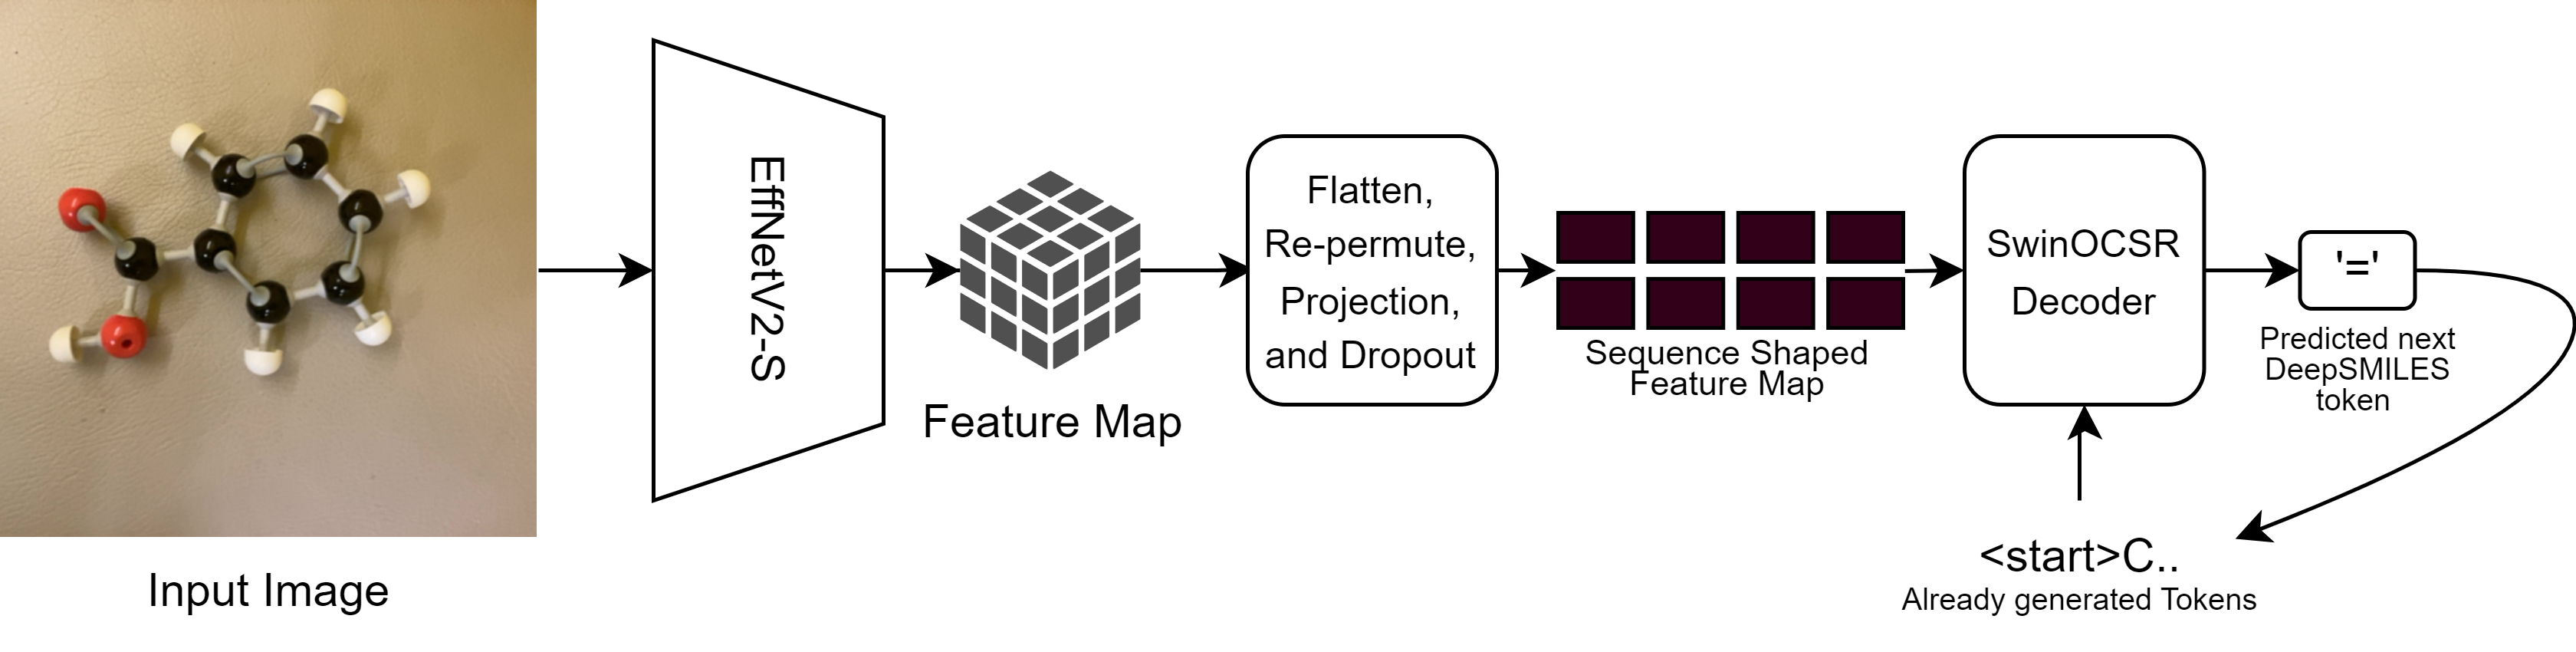
\includegraphics[width=0.9\textwidth]{arch}
    \caption{Model Architecture}
    \label{fig:arch}
\end{figure}

Our model architecture is shown in Fig \ref{fig:arch} and is very similar to the ones used in DECIMER.ai \autocite{decimer} and SwinOCSR \autocite{swinocsr}. The encoder we used is the EfficientNet-V2-S \autocite{effv2} from torchvision \autocite{torchvision2016} with internal parameters that are trained on ImageNet-1k \autocite{imagenet}. The reason behind selecting EfficientNet-V2-S instead of SwinTransformer like in SwinOCSR \autocite{swinocsr} is that on TorchVision the EfficientNet family actually has higher accuracy, and the reason for selecting the S (small) version of the EfficientNet-V2 is due to the very limited data in the fine-tuning real-world dataset: it will be beneficial to choose a smaller model to avoid overfitting. 

We extracted all the convolution layers from the EffcientNet-V2-S to get a feature map with size $1280\times13\times13$ ($Channel \times Width \times Height$)  for each batch. This feature map is then flattened into 2D shape $1280\times169$, re-permuted to sequence-like shape $169\times1280$ ($Sequence \times Channel$), projected to 256-dimension to match the input shape of SwinOCSR decoder, and passed through a dropout layer. The tensor is then fed into our decoder. which is adapted from SwinOCSR \autocite{swinocsr}. We also used focal loss in our model; however, instead of sigmoid, we used Softmax as implemented in \cite{torch_focal}.

During training, we use the ``teacher forcing" method: the model will be given all the correct tokens and for each token ($t$-th) the model will predict the next token $(t+1)$-th on the same position on the output. Since the decoder in Transformer is masked self-self-attention, the token at $t$ will only have an attention score with previous tokens ($0\dots t-1$). This utilizes the parralization feature of the Transformer. However, this makes the model only see the correct previous tokens and not the wrong previous tokens (which would be common during inferences), making it possible for the model to cumulate the mistakes during inferences. \autocite{bengio_scheduled_2015} Thus, scheduled sampling \autocite{bengio_scheduled_2015} proposed to sometimes use the model's own output as the \textit{previous tokens} during training. However, this will disrupt the parallel features of transformers. Additionally, unlike natural language, which has some variation and fault tolerance, the DeepSMILES we generated has only one correct answer. Thus, it does not matter if the error is cumulative as the DeepSMILES would be wrong either way. Therefore, we are not using the scheduled sampling in this project. 

\subsection{Beam search and Multi-image input}
Beam search is a way to increase the accuracy of autoregressive models. \autocite{yang_breaking_2018} \autocite{zhang_beam_2024}. Beam search can also provide users with multiple candidate answers to choose from, similar to the top-$n$ in image classification. However, one issue with beam search is that it will favour shorter sequences as a sub-sequence will always have a higher probability than its parent sequence. \autocite{yang_breaking_2018} \autocite{zhang_beam_2024} There are multiple methods to solve this issue, some are mentioned in \autocite{yang_breaking_2018} and \autocite{zhang_beam_2024}. In this paper, we use a simple method mentioned in \autocite{zhang_beam_2024} where we multiple $\frac{1}{L^\alpha}$ to the log probability where $L$ is the length of the sequence. This will make the log probability of a long sequence higher (since the log probability is negative). It can also be seen as taking the mean of the $logprob$ of each token when $\alpha=1$. The re-scored $logprob$ is shown in Equation \ref{beam}.\cite{zhang_beam_2024} where $P(y_t|y_1\dots y_{t-1}, \textbf{e})$ is the probility of output $y_t$ at $t$-th token given pervious tokens $y_1\dots y_{t-1}$ and image embeding $\textbf{e}$. 
\begin{equation}
    LP = \frac{1}{L^{\alpha}}\sum_{t=1}^{L}logP(y_t|y_1\dots y_{t-1}, \textbf{e})
    \label{beam}
\end{equation}
% In this project, we set \(\alpha=0.75\) as suggested in \autocite{zhang_beam_2024}. 

Additionally, we also hypothesize that multiple image inputs will increase the accuracy of the model. This has been shown in previous research \autocite{sun_multi-input_2017}, in which the authors use the ``early fusion" method where feature maps from 3 different images are concatenated on the channel axis in the early stage of the network. However, this method requires modification of the backbone network and the number of images in this method is fixed. Instead, our method passes individual images through the entire network (including the EfficientNet-V2-S and SwinOCSR decoder) and averages the softmax distribution of tokens, as shown in Equation \ref{eq:mi} where $I$ is the input image set, $M$ is the model, $P(y_{t,j})$ is the probability of token $j$  at time $t$, and $\sigma$ is the Softmax function. The comparison of our models and \autocite{sun_multi-input_2017} is shown in Figure \ref{mi}. 
\begin{equation}
    P(y_{t,i})=\frac{1}{|I|}\sum_{i\in I}P(y_{t,i}|y_0 \dots y_{t-1}, i) = \frac{1}{|I|}\sum_{i\in I}\sigma(M(y_0 \dots y_{t-1}, i))
    \label{eqmi}
\end{equation}
\begin{figure}
    \centering
    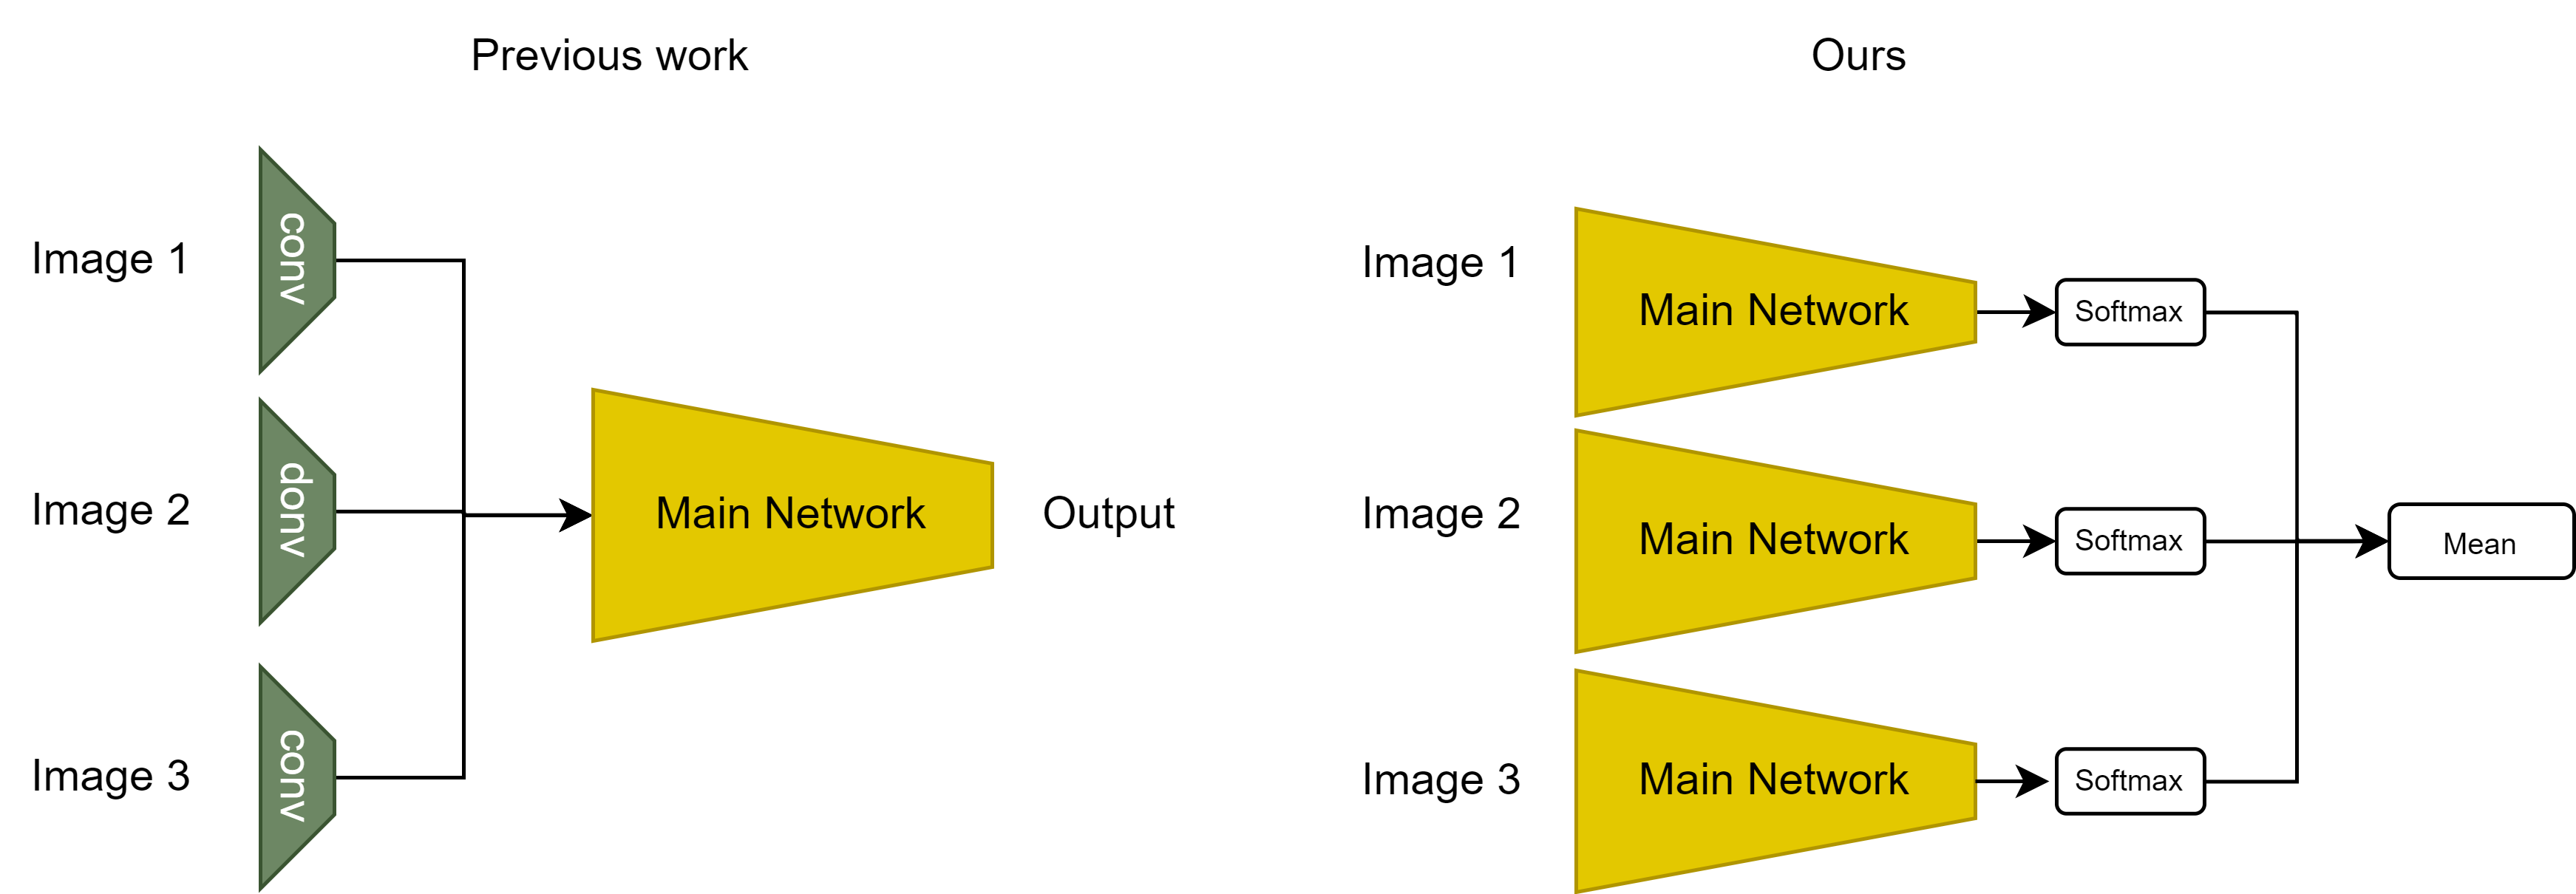
\includegraphics[width=0.8\textwidth]{mi.drawio.png}
    \caption{Muti-Image Input Apporch of Pervious work \autocite{sun_multi-input_2017} and Ours}
    \label{mi}
\end{figure}


\subsection{Improve Accuracy By Self-Reflection}
%should i put this in related works
It has been shown that in Large Language Models (LLMs), it might be hard for the model to output useful and safe information, but it is easy for the model to find it after re-evaluating it. \autocite{bai_constitutional_2022} Similar ideas have been shown in some image-text generative models such as DALL-E \autocite{ramesh_zero-shot_2021}
% and 
% CLIPasso \autocite{vinker_clipasso_2022} 
where another model (in these two cases, CLIP \autocite{radford_learning_2021}) is to evaluate multiple outputs of the generative model and select the best output in the generated. There are also some image-text matching evolution metrics being proposed such as CLIPScore \autocite{hessel_clipscore:_2022} and image-text matching loss \autocite{xu_attngan:_2017} to evaluate the similarity between text and image. 

However, CLIP is a contrastive learning model: for a given number of image-text pairs, the feature of each image and text is extracted by its corresponding encoder, and then in the embedding space, it is treated as a multi-class classification problem to match each image with corresponding text. \cite{radford_learning_2021} Thus, it usually requires a large number of negative samples (32,768 in \autocite{radford_learning_2021}) in the batch for the model to learn useful information. \autocite{he_momentum_2020} Although there are models like Momentum Contrast  (MoCo) \autocite{he_momentum_2020} to build a large negative sample queue using a smaller batch size by momentum for pure image tasks, it is hard to use such strategy for multi-modality tasks involving both text and images without adding complexity to the model or training pipeline. 

Image-text matching loss (being used in many multi-modality models, such as \autocite{li_align_2021} \autocite{liao_evaluation_2023}\autocite{xu_attngan:_2017}), on the other hand, does not treat this problem as a multi-class classification problem but a binary classification problem. That is, for each pair of images and text, the model needs to determine if it is a matched pair. This method does not require a large batch size and can be trained on a single GPU. The models we used involving a transformer decoder, unlike \autocite{li_align_2021} and \autocite{kim_vilt:_2021} which use the transformer encoder, we put the feature extraction token at the end of the sequence, like in Generative Pre-trained Transformer-1 (GPT-1) \autocite{alec_improving_nodate}. Specifically, when the model outputs the \verb|<end>| token, this will be appended to the \textit{generated sequence} same as other tokens, and when the model gets this token as input, the output of the last layer of the transformer will not be projected to predict tokens but projected to do a binary classification for image-text matching using a two-layer MLP. This process can be found in Figure \ref{fig:itm}.

\begin{figure}
    \centering
    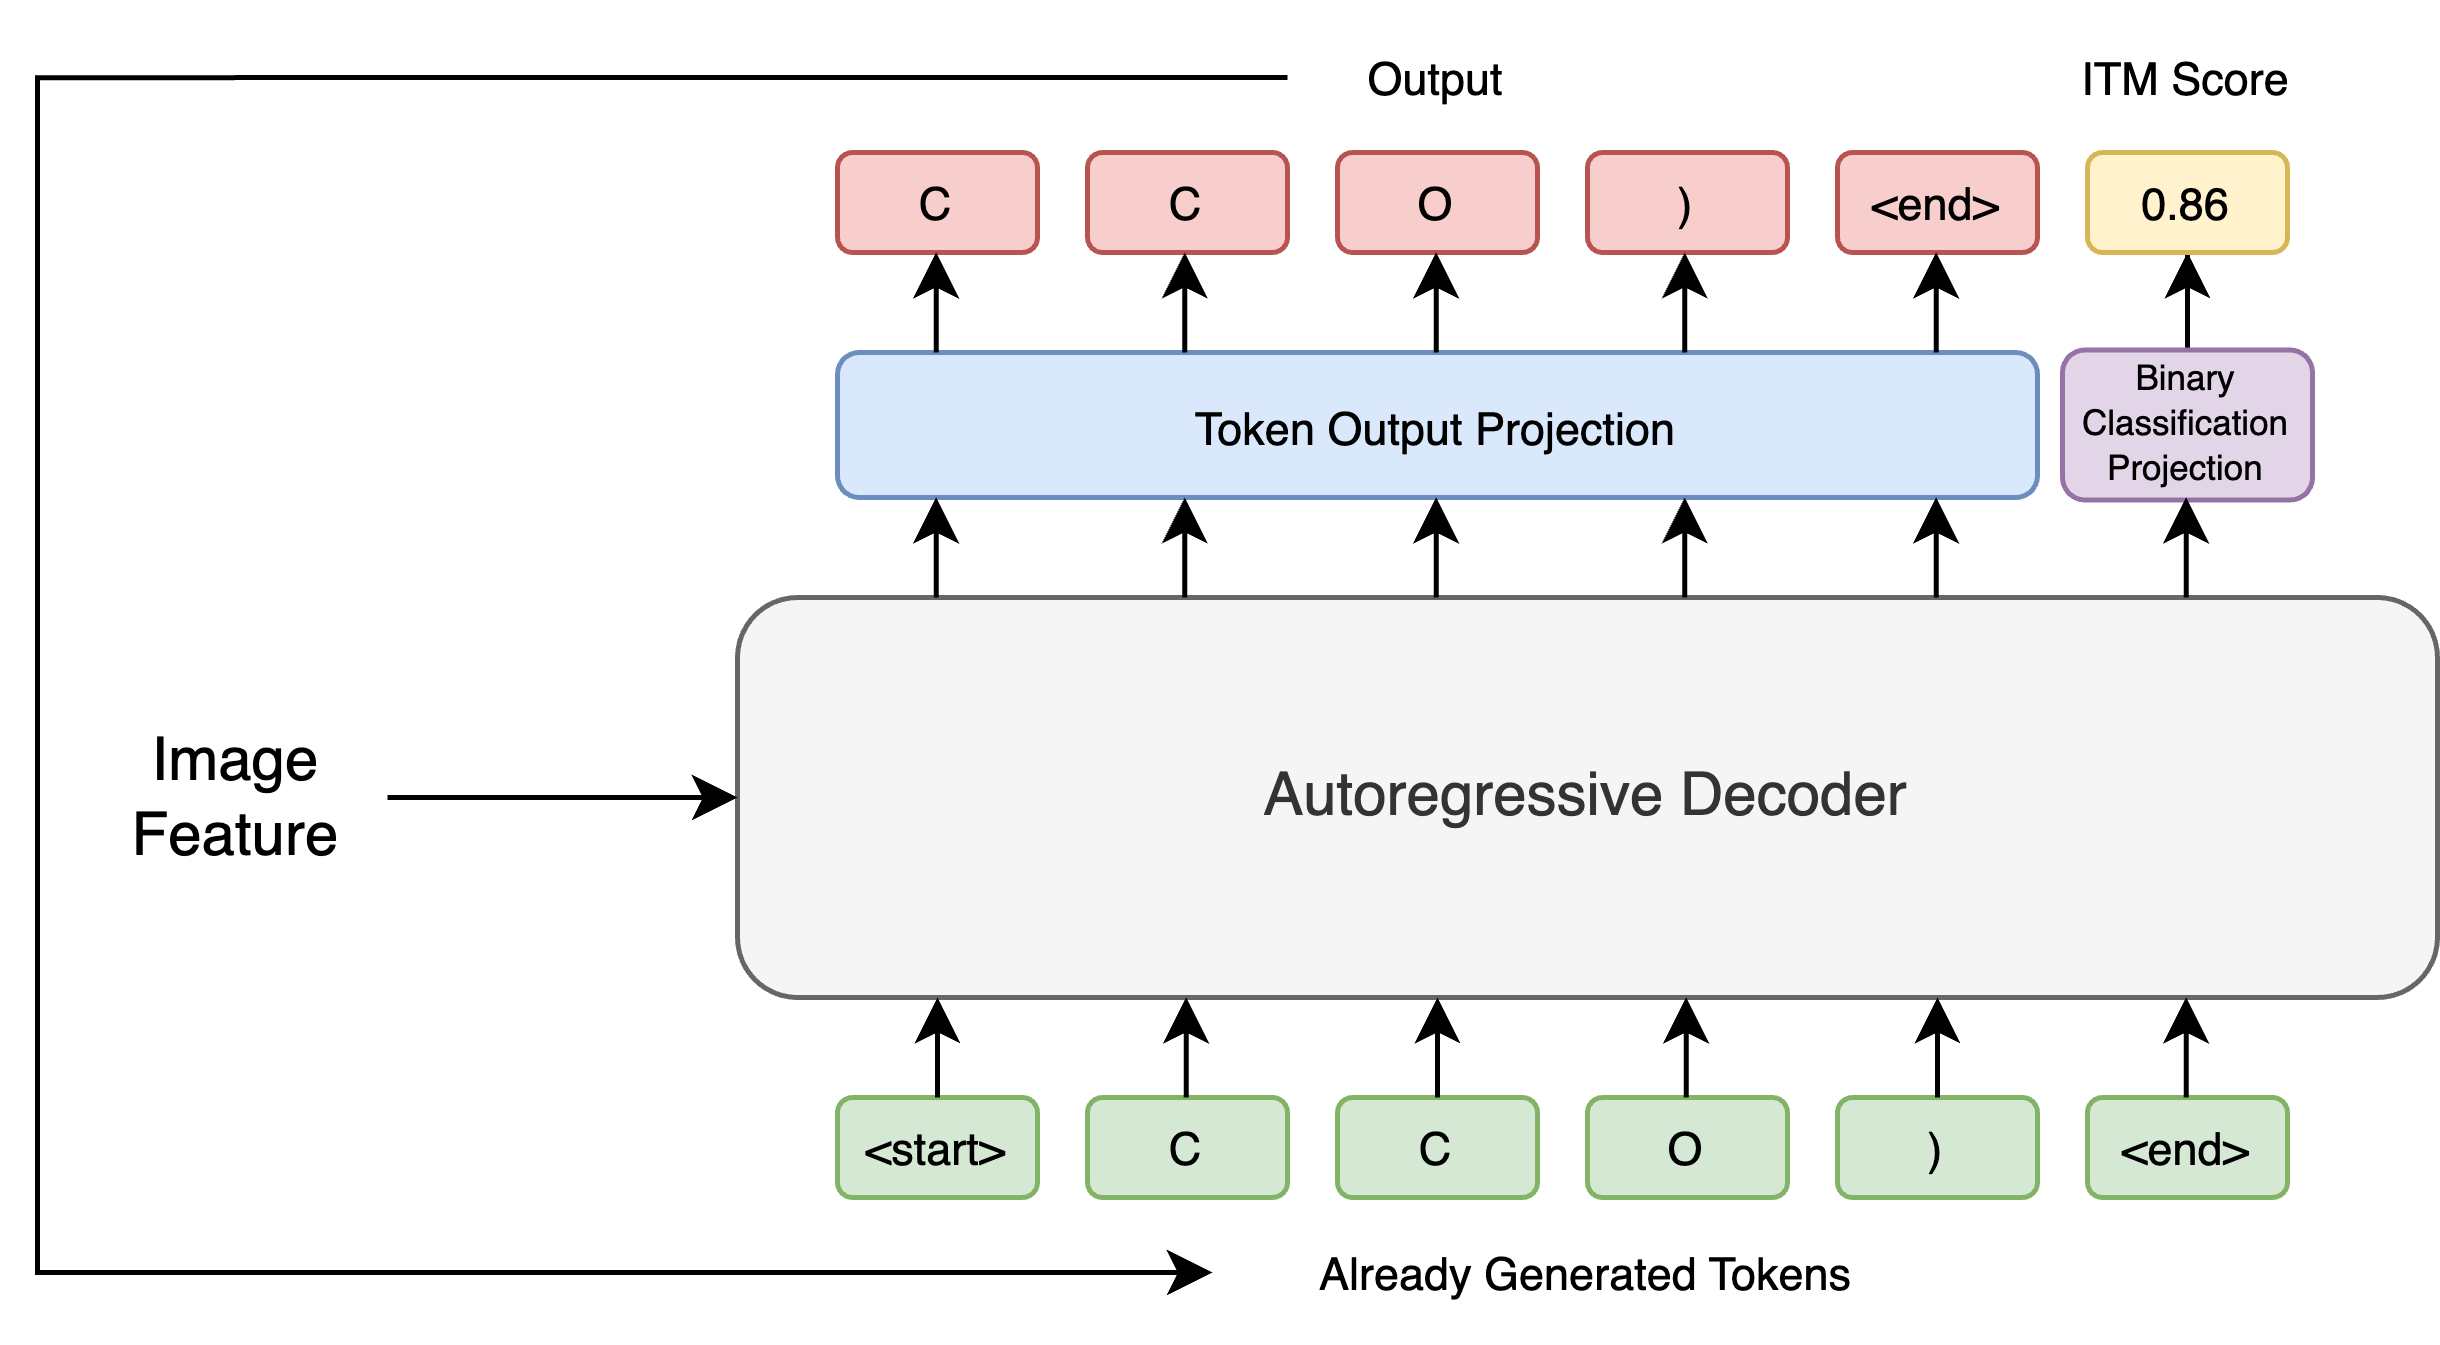
\includegraphics[width=0.8\linewidth]{itm.drawio.png}
    \caption{Model With Image-Text Matching}
    \label{fig:itm}
\end{figure}
Since the purpose of the ITM score is to find the best sequence in multiple model-generated sequences, it will be beneficial to use the model's mistakes as negative examples in ITM training. To achieve this, we maintain a dictionary with the values are queues of recent wrong model-generated output and keys are the correct answer. At the beginning, the queue is initialized with random DeepSMILES strings in the training (we did not exclude the correct answer because it will add computational overhead and the chance of selecting the correct answer in it is very low) set and progressively replaced by the model output. By using this method, the model can learn from its own mistakes. This task will also get progressively more difficult because as the model trains, its output will get more similar to the correct answer even when it is wrong. This process is shown in Figure \ref{fig:selfnegative} and the pseudocode can be found in Listing \ref{selfnagative}, detail such as translating between tokenized sequences and DeepSMILES, removing special tokens, reshaping, are not included.   
\begin{figure}[t]
    \centering
    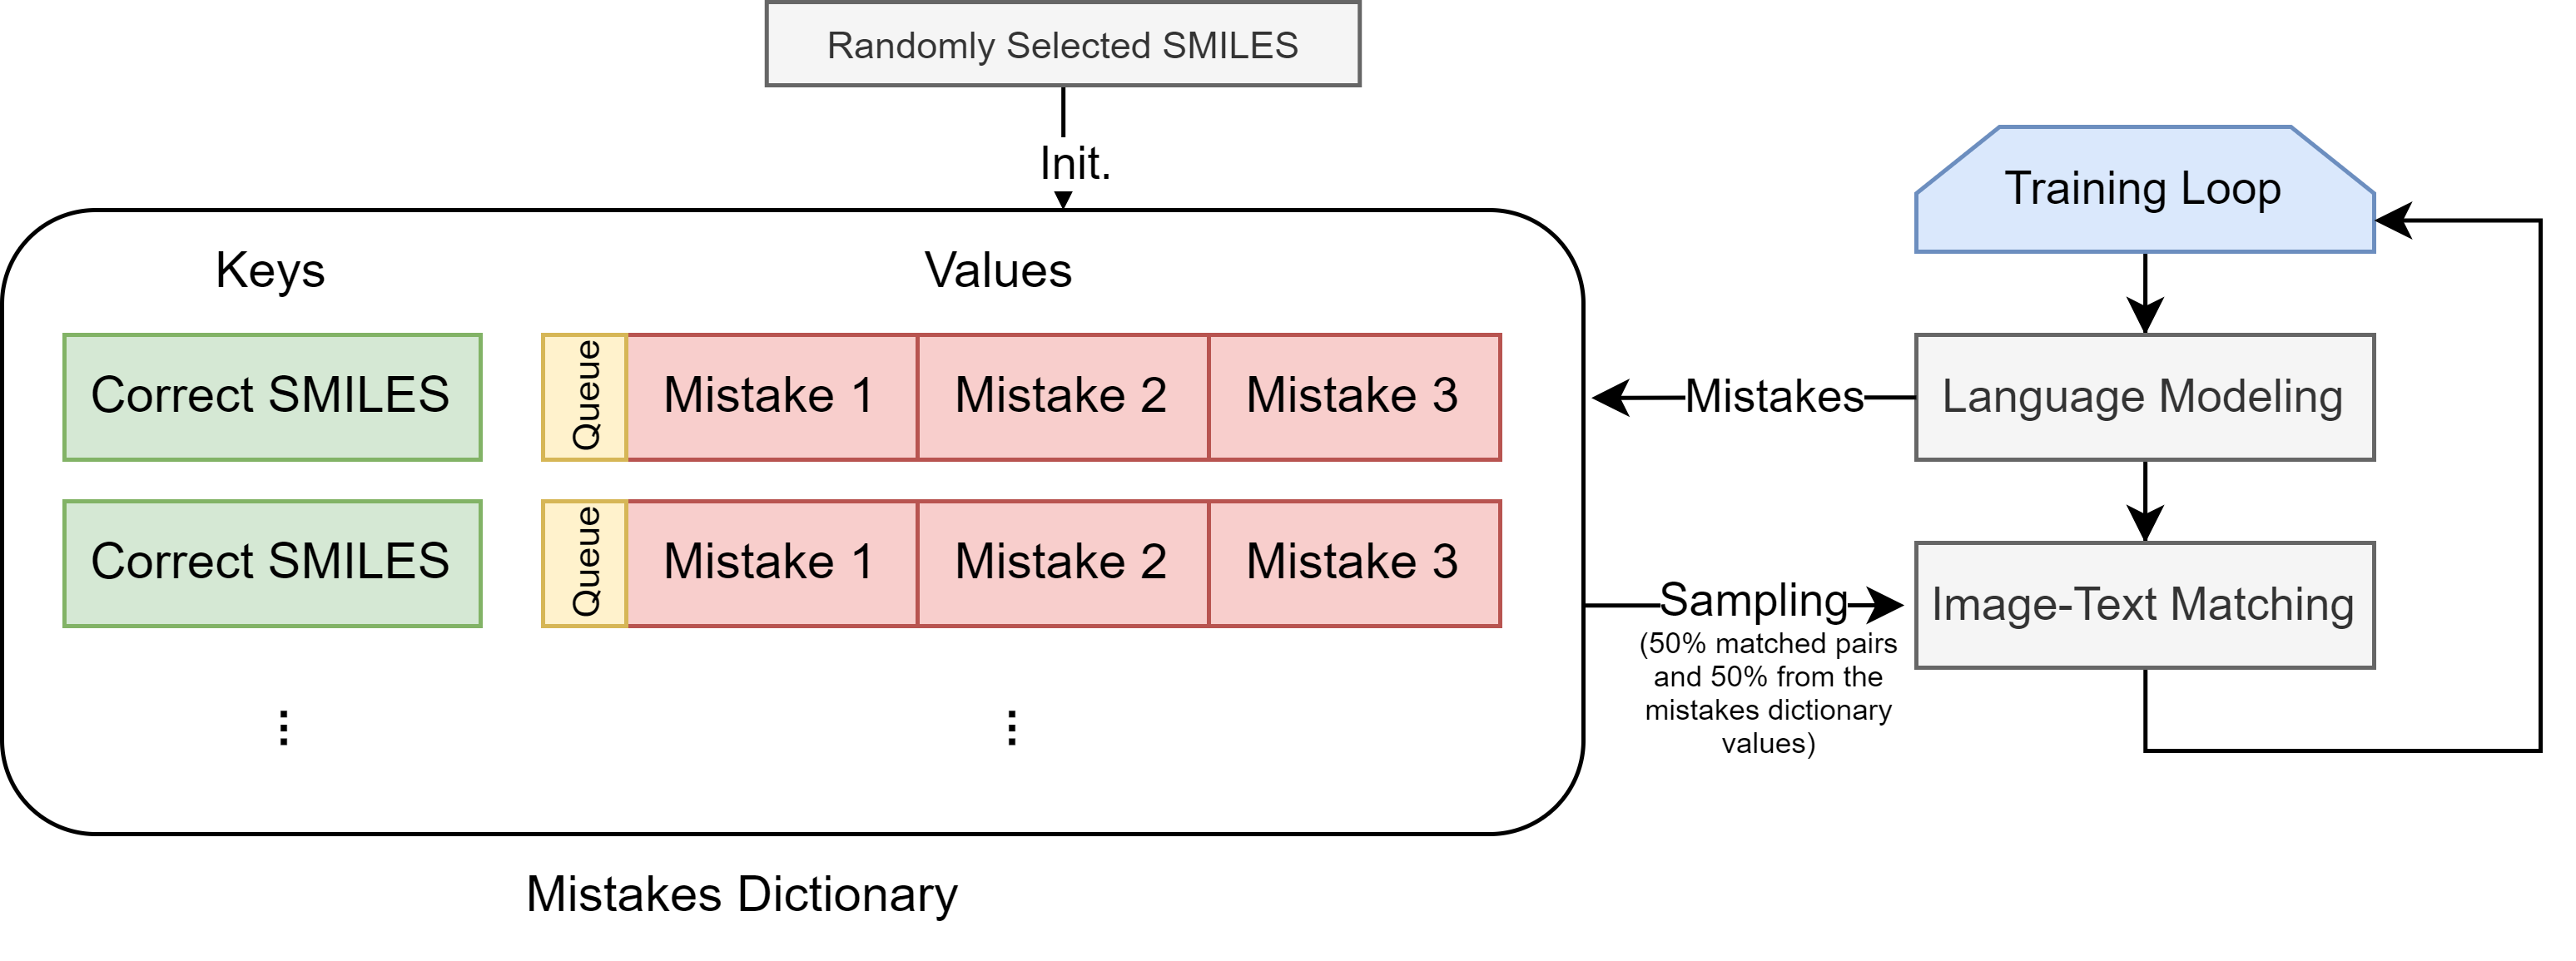
\includegraphics[width=0.8\linewidth]{selfnegative.drawio.png}
    \caption{Mistakes Dictionary and Self-Negative}
    \label{fig:selfnegative}
\end{figure}
\begin{minipage}{\linewidth}
\tiny

    \begin{lstlisting}[language=Python, caption=Training Process Pseudocode, label=selfnagative]
mistakes = {correct:random.choices(SMILES, k=3) for correct in SMILES}

# training loop
for img, text_in, text_out, epoch in dataloader():
    # text_in is <start>SMILES<end>, text_out is SMILES<end>
    outputs = model(image, text_in, predict = True)[:,:-1,:]
    loss = focal_loss(outputs, text_out)
    model.gradient_descent.step()
    if max_epoch - epoch <=3
        for i in range(BATCH_SIZE):
            if outputs != text_out:
                mistakes[text_out[i]].append(outputs[i])
                mistakes[text_out[i]].pop(0)
        
        label = [random()<0.5 for _ in range(BATCH_SIZE)]
        text_in = [text_out[i] if j else random.choice(mistakes[text_out[i]]) for i, j in enumerate(label)]
        # predict = False for binary classification 
        outputs = model(image, text_in, predict = False)
        # * 1.2 to give ITM loss more weight
        loss = binary_cross_entropy_with_logits(outputs, label) * 1.2 
        model.gradient_descent.step()
    
\end{lstlisting}
\end{minipage}
    % for i in range(BATCH_SIZE):
    %     corr = text_out[i]
    %     if random.random()<0.5:
    %         text_in.append(corr)
    %         label.append(1)
    %     else:
    %         text_in.append(random.choice(mistakes[corr]))
    %         label.append(0)
\subsection{Experiment}
\begin{figure}
    \centering
    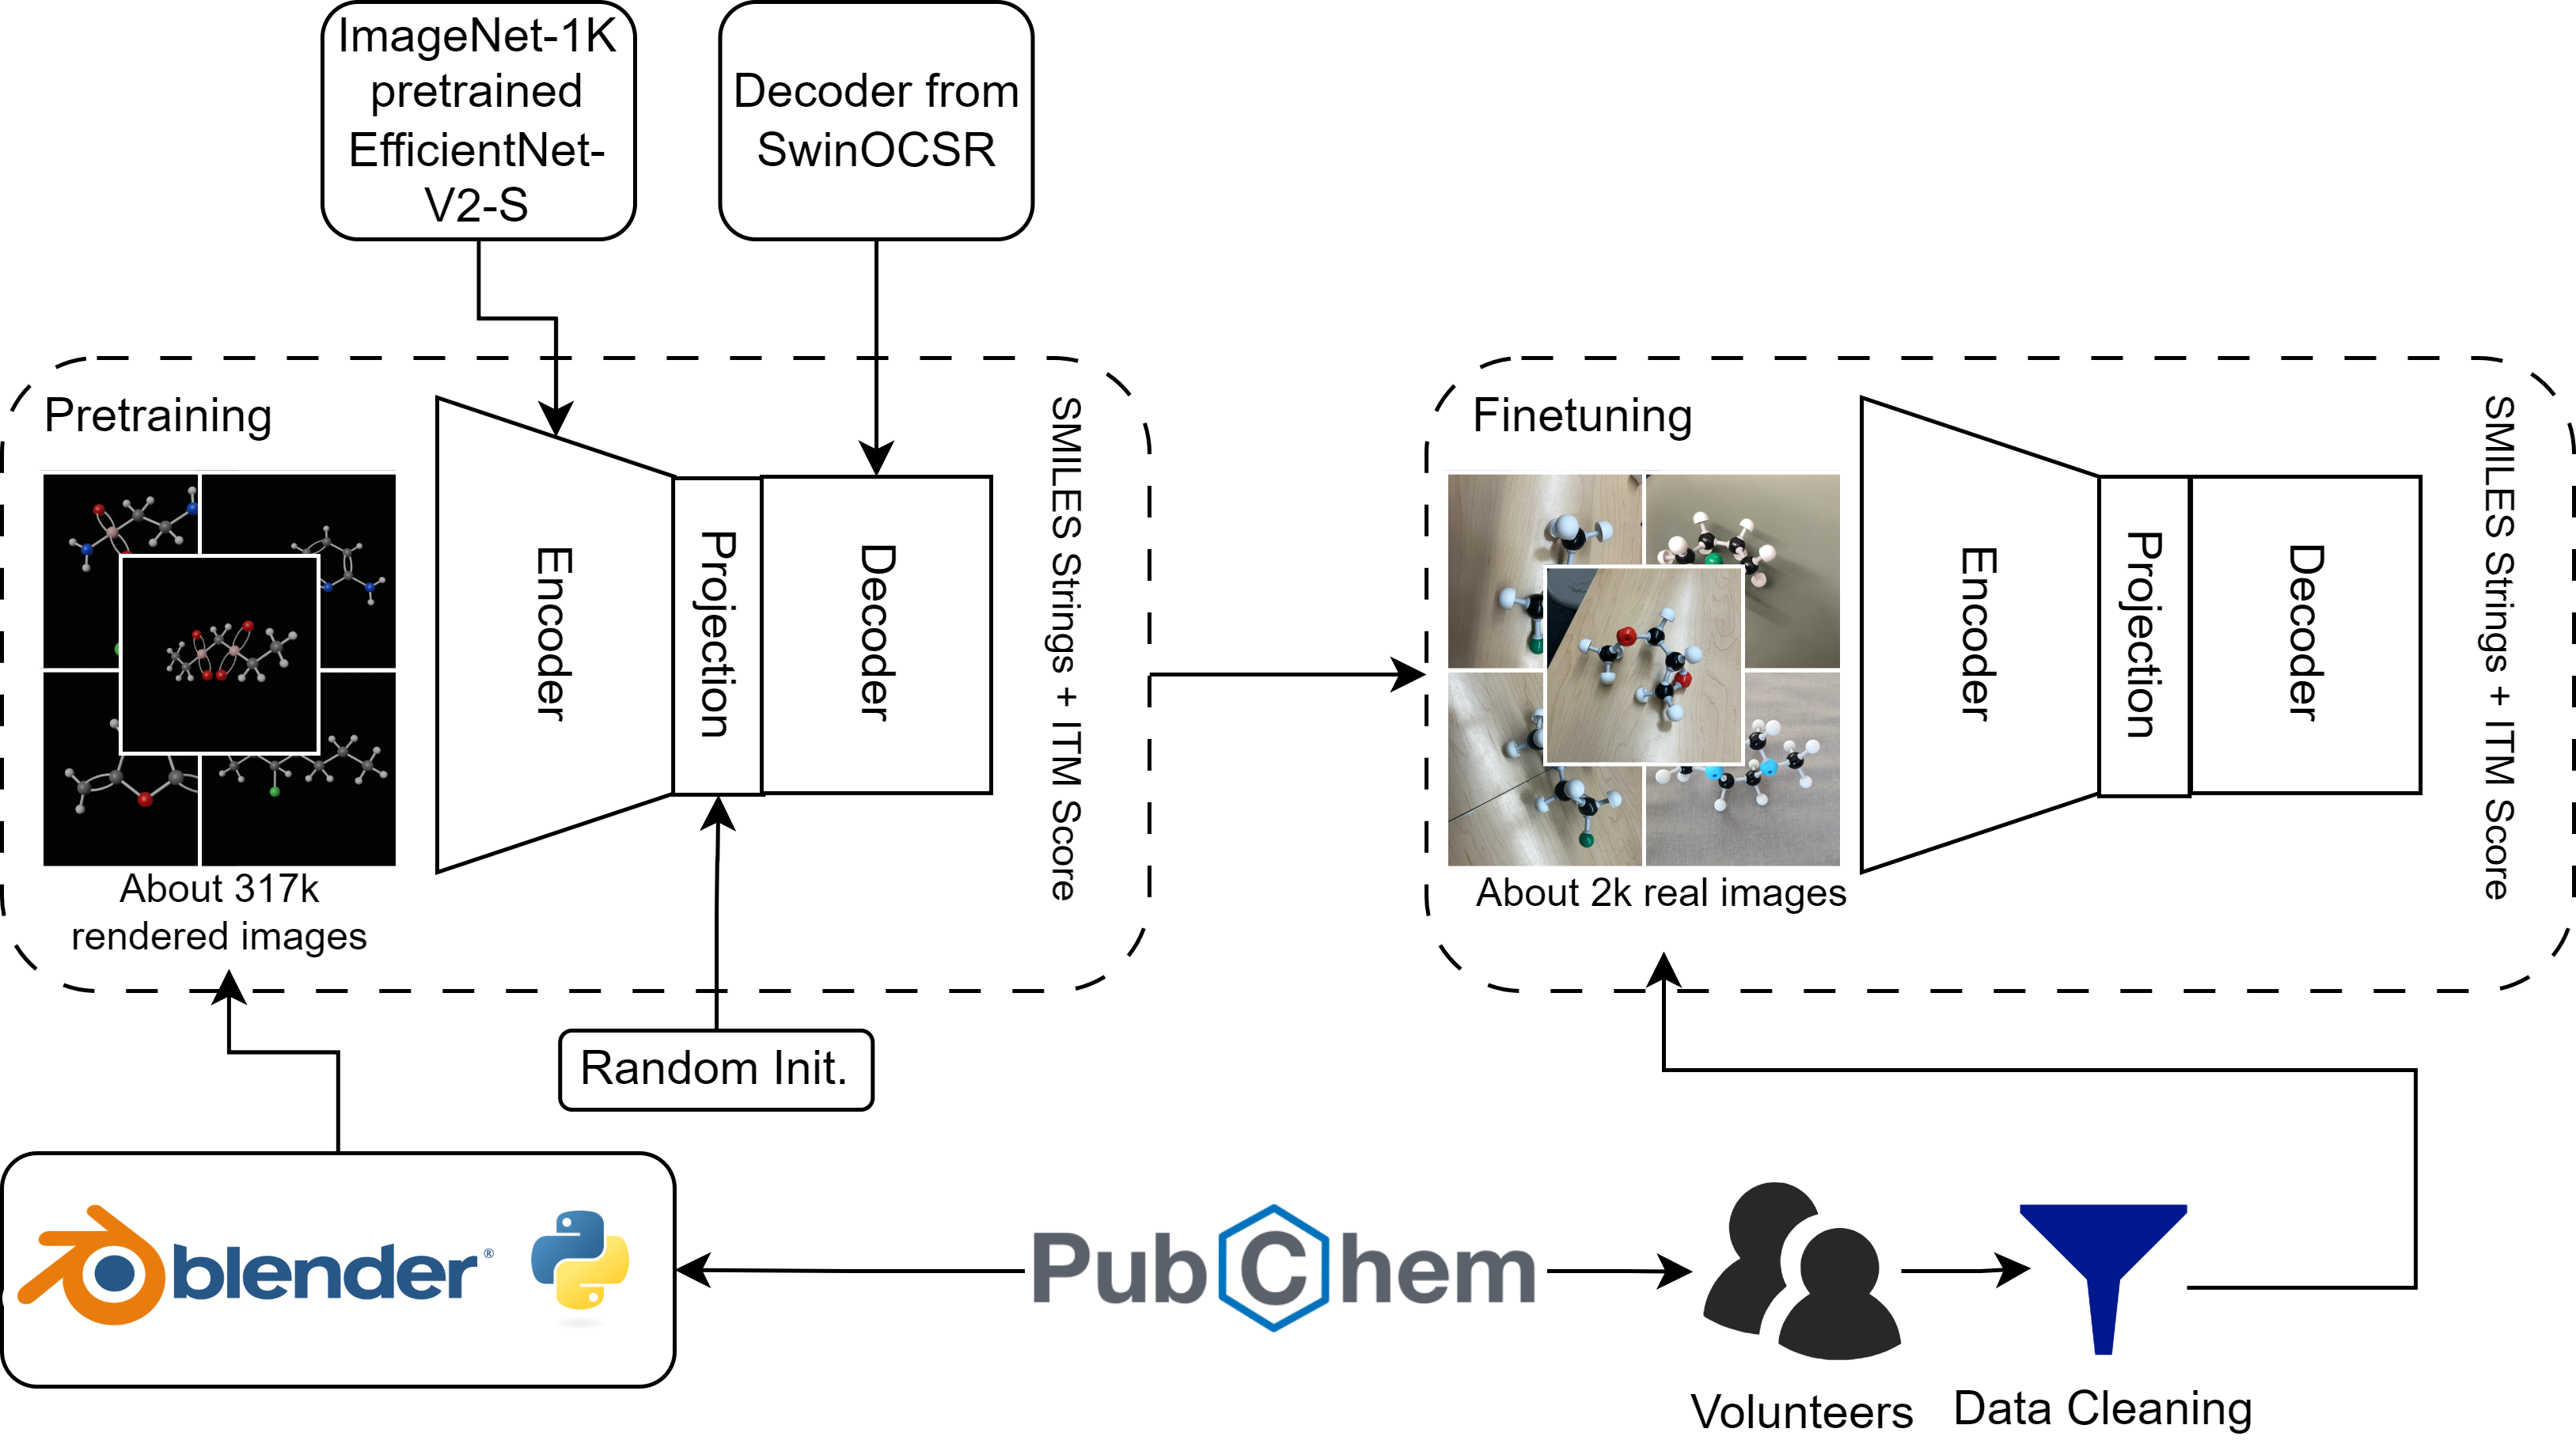
\includegraphics[width=0.5\linewidth]{pipeline.png}
    \caption{Training Pipeline}
    \label{fig:pipeline}
\end{figure}
Since we have a small dataset for fine-tuning, we applied many random online data augmentation during the training process: random rotation, random flipping, random cropping,  and random colour jitter (including RGB channels and brightness). 

We train our model on the synthetic dataset with AdamW \autocite{adamw} and an exponential learning rate scheduler. We then fine-tune our model on the real-world dataset. The training pipeline of the model is shown in Figure \ref{fig:pipeline}. For the model with ITM, during pretraining, the two loss functions (language modelling and image-text matching) are used at the same time throughout the whole process. A backward propagation and gradient descent step is performed after each forward for each loss function. However, during fine-tuning, the ITM loss is only used in the last 2 epochs. 
With the fixed validation set, we did a hyperparameter search using both Weight and Bias \autocite{wandb} and manual tuning to select models with the highest validation token-level accuracy.  
% Similar to the pretraining, the decoder is frozen. 
% Additionally, we also freeze the projection layer between the encoder and reladecoder and the last 2 blocks of encoder EfficientNet-V2-S since the input of the decoder is in the same domain for pre-training and finetuning. This could also decrease the number of trainable parameters to avoid overfitting. 
After training, we tested the model on a dataset between validation and testing. This dataset is not used in finetuning the hyperparameters but is used to test after hyperparameter tuning. However, it is not the final testing set. If the model performance is not ideal on this dataset, we returned the hyperparameters. This intermedia dataset could be used multiple times and will be merged into the validation set at the end and the model will be tested on a real dataset
.
\section[Results and Discussions]{Results and Discussions\footnote{Although there are variations between each training, we only take one trained model in the evolution for simplicity. And different parts of the result might use different trained models. }}
\subsection{Accuracy}
We extended our validation set with some more molecules, this dataset is also filtered to remove images with occlusion and bad lighting. However, we kept some images that could be out of the domain for the model (poor lighting but atoms are still visible, and overly simplified molecule: methane) to avoid biased results from cherry-picking the data. For each molecule, take $k$ samples where $k$ is the number of images for that molecule in the dataset. For each sample, we randomly select $N$ images from the dataset without replacement. With a fixed $\alpha=0.75$ and softmax temperature $t=1$, the top-1 and top-$n$ sequence-level accuracy is shown in Figure \ref{grid}. 

\begin{figure}
    \centering
    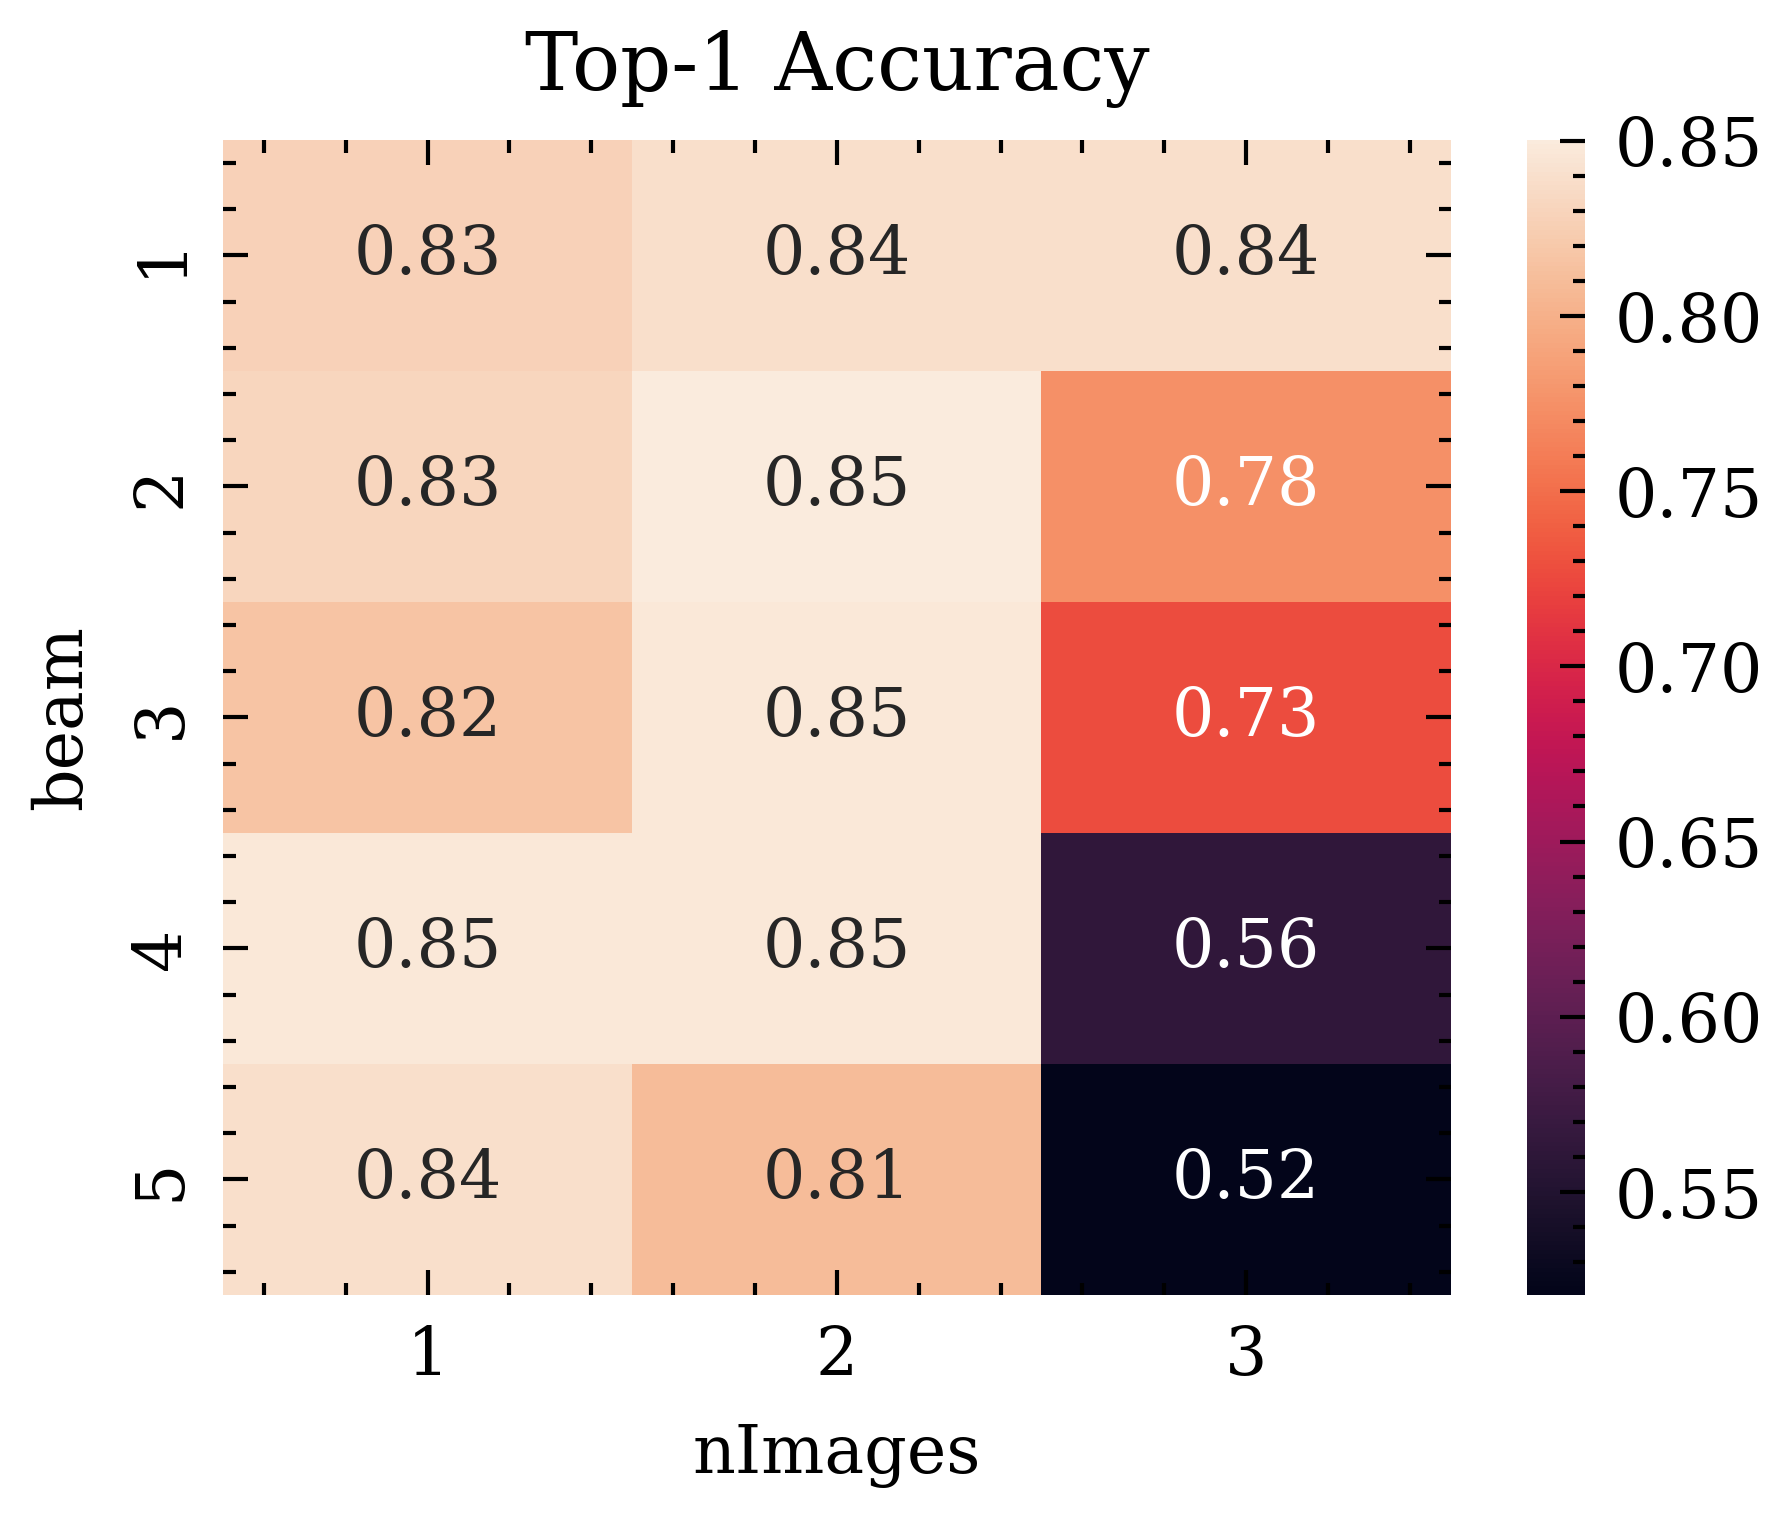
\includegraphics[width=0.45\linewidth]{top1.png}
    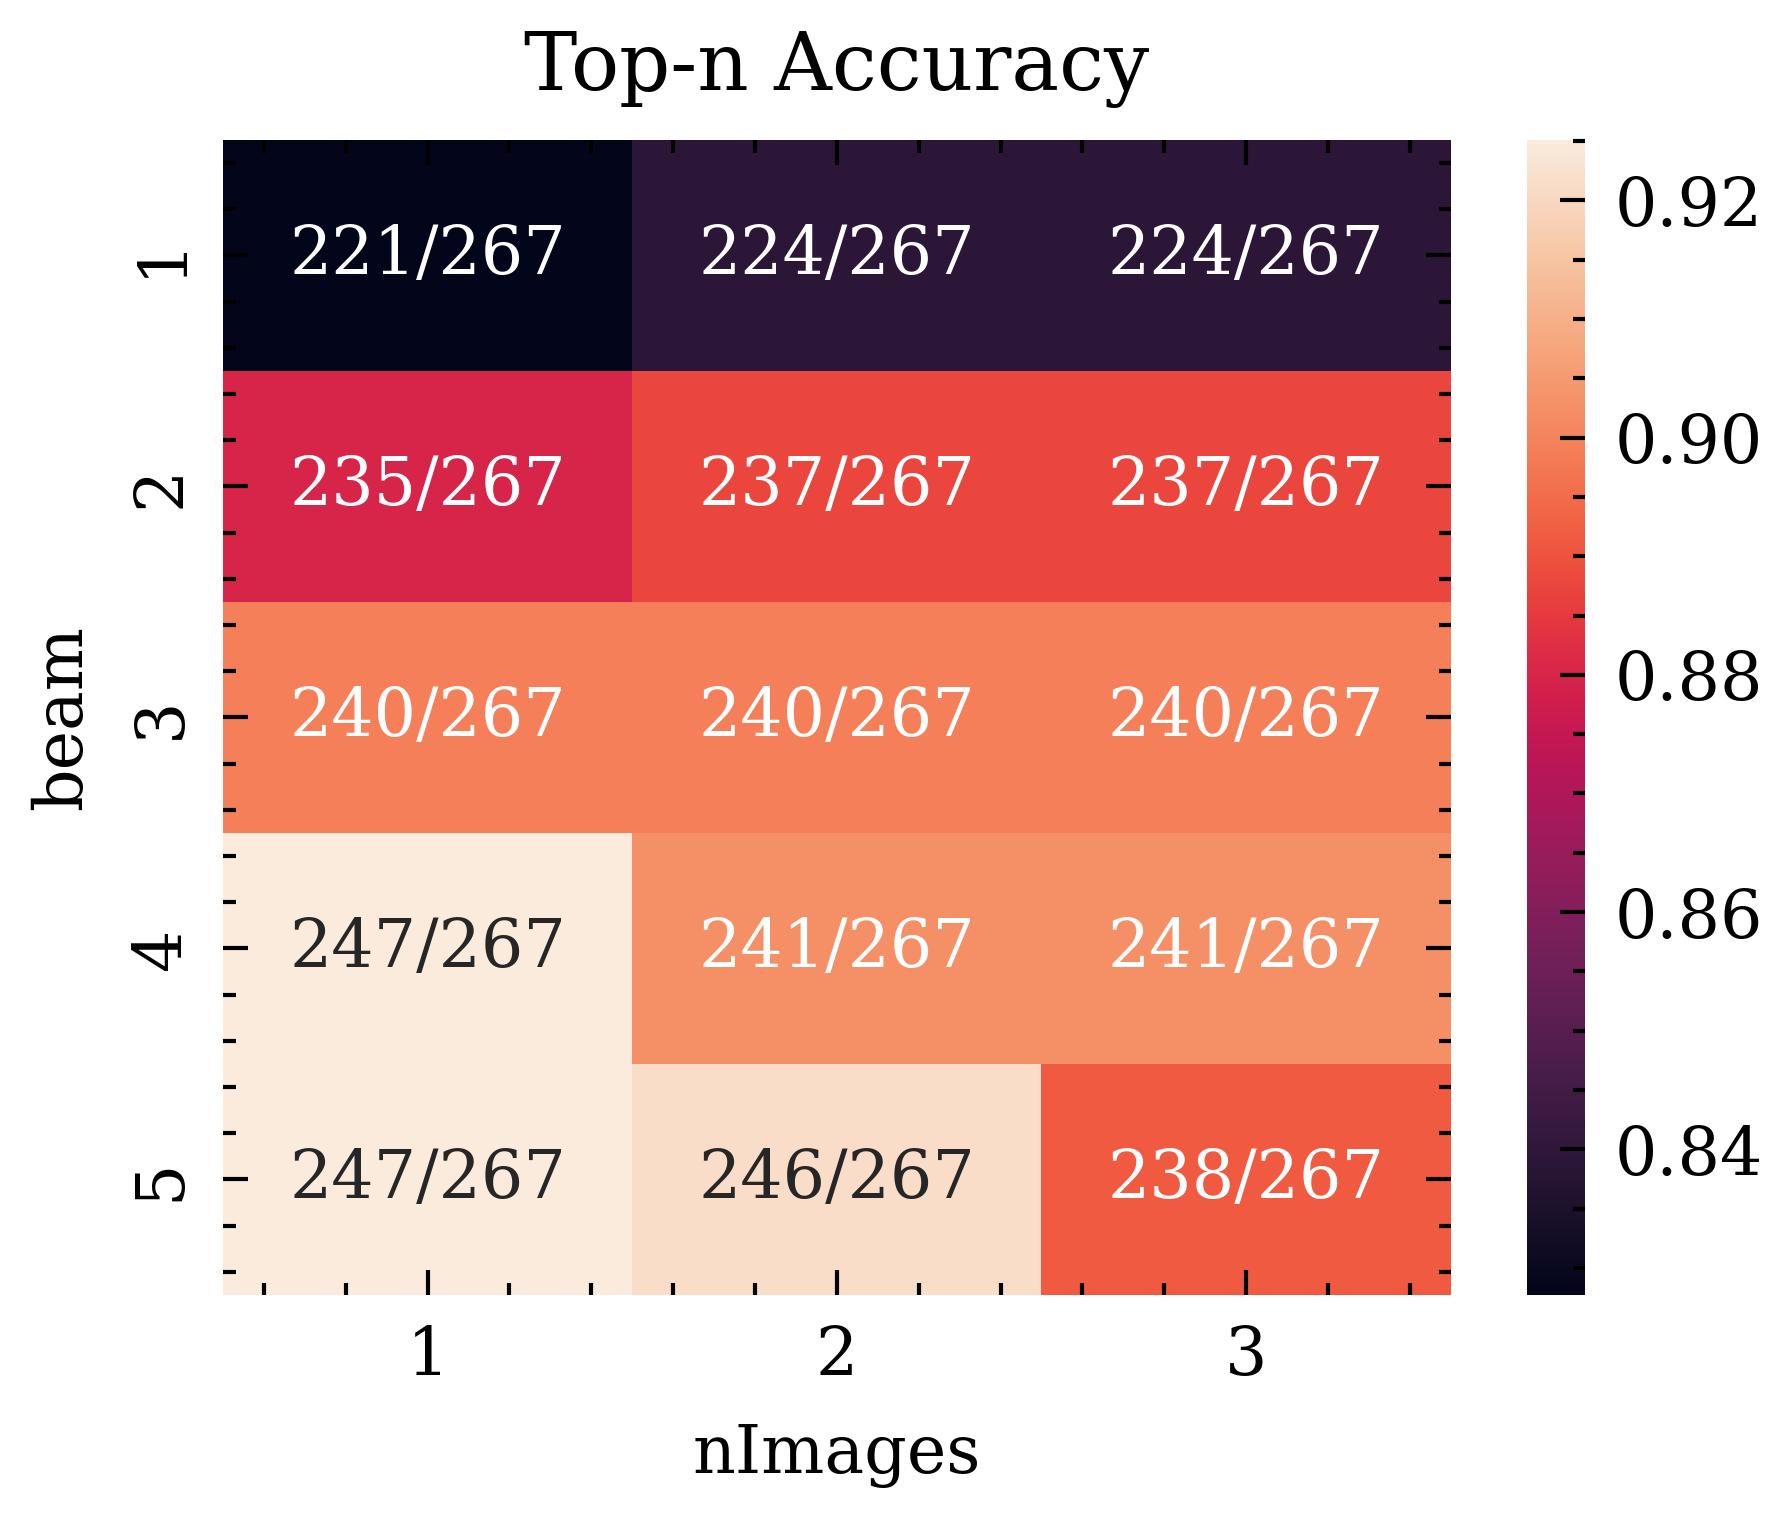
\includegraphics[width=0.45\linewidth]{topn.png}
    \caption{Model Accuracy with Fixed $\alpha$ and $t$}
    \label{fig:grid}
\end{figure}

Similar to \cite{swinocsr}, we evaluated the relationship between our model's performance with types of molecules and smiles string length. However, since our validation dataset is extremely limited, this could not be used as a defined answer. Figure \ref{fig:acc_each} shows the accuracy of each molecule in the validation set of the model without ITM. We can observe that for a few molecules, even the complex ones like caffeine, the model can achieve 100\% accuracy on them. However, on the other hand, there are a few molecules that the model achieves 0\% accuracy. A list of these molecules and their sample images are included in the Appendix. We also examined the relationship between the length of DeepSMILES and the accuracy as shown in Figure \ref{lenacc}. We can observe that there is no significant relationship between the DeepSMILES length and accuracy ($p=0.527$). This could indicate that the difficulty of a molecule does not depend on its length, but could also be due to the limited validation set size.  

\begin{figure}
    \centering
    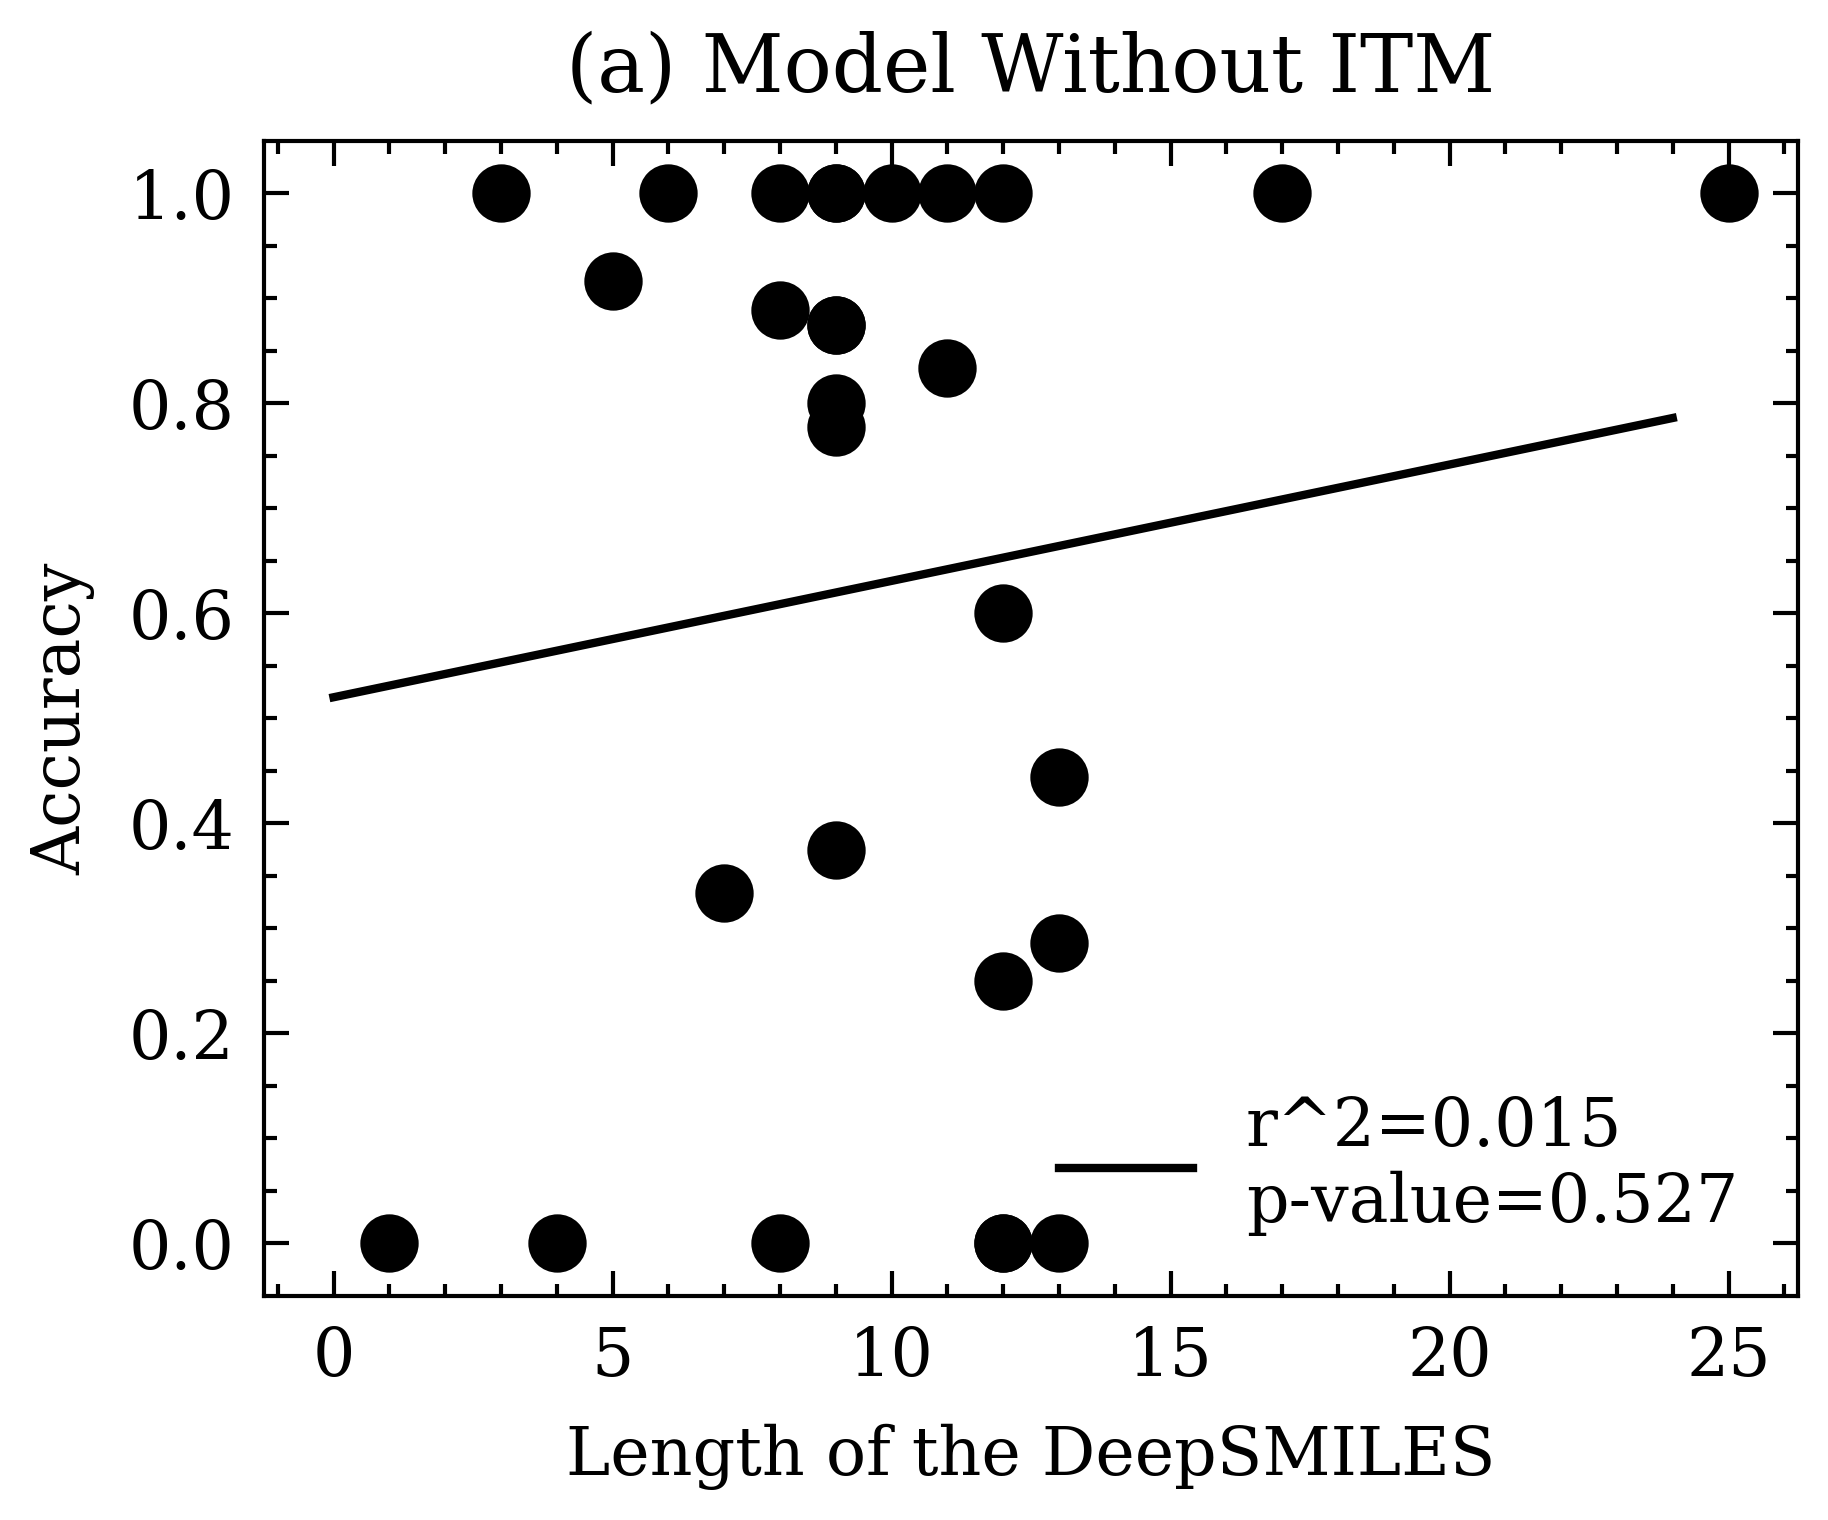
\includegraphics[width=0.5\linewidth]{lenacc.png}
    \caption{Relationship Between Length of DeepSMILES and Accuracy}
    \label{lenacc}
\end{figure}


% \begin{equation}
% S = P_{1} + 0.9P_{n}
% \label{score}
% \end{equation}

% \begin{table}[]
%     \centering
%     \begin{tabular}{c|cc}
%       $beam$ & Top-1 Accuracy & Top-$beam$ Accuracy \\ \hline
%       1 & 71.9 ± 5.8 & 71.9 ± 5.8 \\ 2 & 72.3 ± 5.8 & 79.8 ± 5.3 \\ 3 & 71.5 ± 5.8 & 84.6 ± 4.9 \\ 4 & 71.2 ± 5.8 & 86.9 ± 4.6 \\ 5 & 71.5 ± 5.8 & 87.3 ± 4.6
%     \end{tabular}
%     \caption{}
%     \label{tab:my_label}
% \end{table}




% Since the above validation set is manually filtered and is used to finetune hyperparameters, it might not be a fair demonstration of our model's capacity Thus, we also tested the model capacity with the hyperparameter found on the validation set on a separately collected testing dataset. And the result of the testing dataset 
% I am not sure what to do here, sweep on test? Do not want to do so: no testing data. alex did not gave it to me. Also i need to find hyperparameter, should i compare it? zhihu said should be on validation 
% In Figure \ref{fig:acc_each}
% compare with hand written OCSR 
% Since to the best of our knowledge, there is no pervious work targeting the same topic, we do not have any benchmark to compare to. However, the DECIMER.ai 

% \begin{table}[]
%     \centering
%     \begin{tabular}{c|cc}
%     nImages & Top-1 Accuracy & top-5 accuracy \\ \hline
% 1 & 65.9 ± 6.4 & 83.5 ± 5.0 \\ 2 & 71.2 ± 5.8 & 85.8 ± 4.8 \\ 3 & 71.5 ± 5.8 & 87.3 ± 4.6 \\  
%     \end{tabular}
%     \caption{Caption}
%     \label{tab:my_label}
% \end{table}
\subsection{Calibration}
The model's calibration is the metric determining if the model's output accuracy is aligned with its uncertify.  The calibration metric of a model is important when it needs to make important decisions such as resume screaming and malware detection. \autocite{liang_holistic_2023} The calibration is important for our sequence generating task for another reason as we will select the output with the lowest uncertainty (highest \textit{logprob}) as the final output. We evaluated our model's calibration using a method similar to \cite{liang_holistic_2023}, we randomly sample in each sample, we randomly select 10 molecules and then randomly select images for each molecule. We calculate the mean accuracy for each sample and the mean perplexity ($logprob$) for each sample and plot them in Figure \ref{fig:cal1} for different $nImages$. Because the sequence probability (perplexity) is the product of the probabilities of each token, the value is usually small, with a range smaller than 0-1. Thus, did not use the commonly used metric expected calibration error (ECE) like in \cite{liang_holistic_2023}. In fact, even in \autocite{liang_holistic_2023}, they did not evaluate the calibration for generative tasks. Instead, we used the $r^2$ value to evaluate the calibration of the model. This is partially inspired by the $r^2$ values used in evaluating the quality of the calibration curve in analytical chemistry (such as absorption or GC-MS). 
\begin{figure}
    \centering
    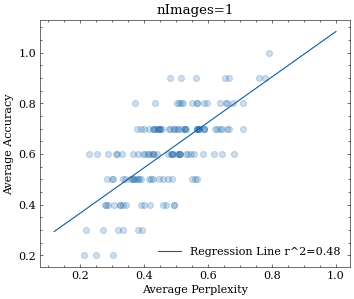
\includegraphics[width=0.3\textwidth]{caln1.png}
    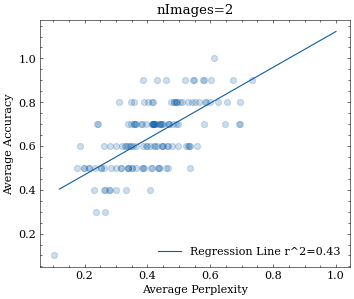
\includegraphics[width=0.3\textwidth]{caln2.png}
    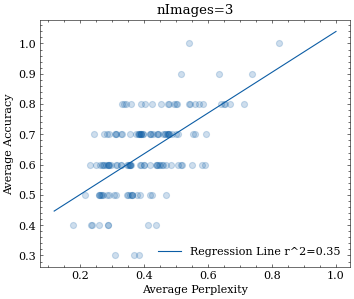
\includegraphics[width=0.3\textwidth]{caln3.png}
    \caption{Calibration Plot of Model Without ITM}
    \label{fig:cal1}
\end{figure}
\begin{figure}[t]
    \centering
    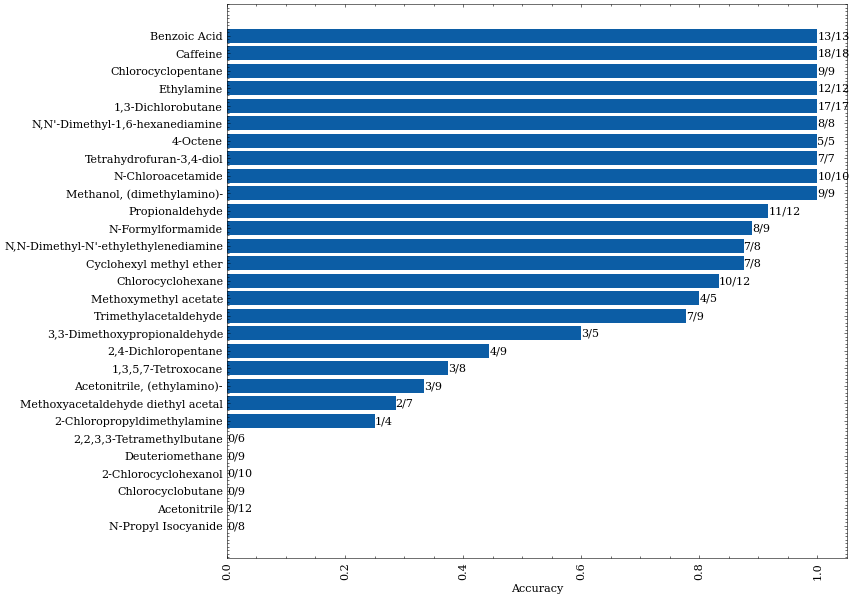
\includegraphics[width=0.8\linewidth]{image.png}
    \caption{Accuracy For Each Molecule}
    \label{fig:acc_each}
\end{figure}
\section{Conclusion}
\section{Demo}
We deployed the model on our server \footnote{\url{http://file.weasoft.com:8888}} with a frontend and open source our model on github\footnote{\url{https://github.com/weathon/3d2smile}}. A simple demo video can be found on YouTube \footnote{\url{https://youtu.be/m4AkzqKC-M4}}. 
\section{Limation and Future Work}
\begin{itemize}
\begin{figure}
    \centering
    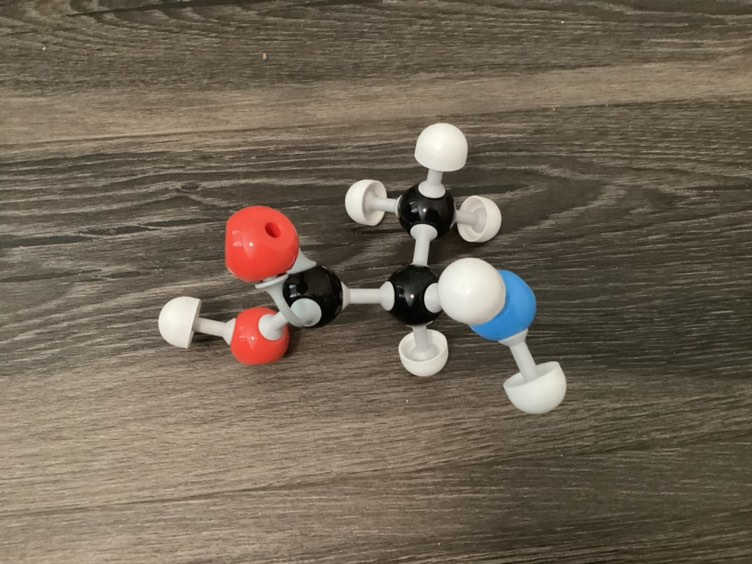
\includegraphics[width=0.3\linewidth]{iso1.png}
    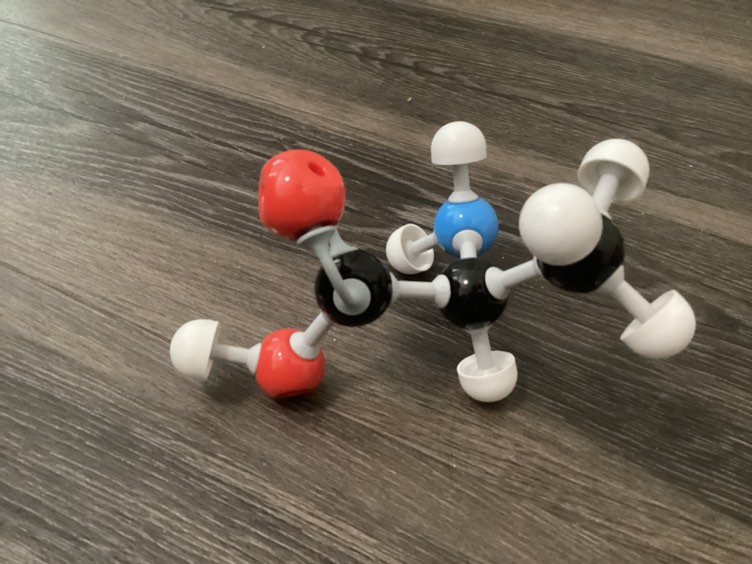
\includegraphics[width=0.3\linewidth]{iso2.png}
    \caption{Stereoisomers Example}
    \label{fig:iso}
\end{figure}

\item In this project, we did not attempt to recognize stereochemical information such as chirality and E/Z structure. However, these are important concepts in organic chemistry for students to understand and being able to show these is one of the key characteristics and benefits of 3D models. However, this is challenging because it requires the ML model not only to understand the connectivity of the atoms but also their relative positions. There are minimal differences between the two stereoisomers. Figure \ref{fig:iso} shows two molecules which are stereoisomers to each other. Additionally, the ML model needs to learn how to output iso-SMILES, which contain stereochemical information, rather than regular SMILES. 
% In future works, we will attempt to recognize the stereochemical information and output iso-SMILES instead of regular smiles. 

\item Both of our datasets are limited by time and budget, especially when compared with previous work such as DECIMER.ai \cite{decimer} and SwinOCSR \autocite{swinocsr} despite our work dealing with real-world photos that have more variations. It is worth it in future studies to collect a larger dataset to increase the accuracy and robustness of the model.

\item This project only focused on the technical side of the problem, including how to collect the dataset, train an ML model on it, and increase the accuracy of the model with various techniques, and did not test how well this application would be in classroom settings, further chemical education studies are needed to determine its effectiveness in education. 

\item Traditional molecular models have some limitations, such as they might be misleading and let students think energy is needed to create bonds when they are not \autocite{snatoms}. Train a machine learning model on alternative molecular models, such as Snatoms\autocite{snatoms}, and might be able to provide better education values. 

\item  The purpose of the mistakes dictionary is to simulate the real mistakes that the model will encounter during inferences. However, during the training, the model generates the sequence by the teaching forcing method while during inferences the previous tokens are generated by the model itself. This will lead to a domain gap between the training mistakes and the inferences mistakes, making it possible that models cannot find the wrong output sequence during inferences. In future work, it is worth investigating if using the model's real output for mistakes dictionary (similar to the idea in Scheduled Sampling \autocite{bengio_scheduled_2015}) will be beneficial. 

\item There are also two other hyperparameters in the inference that we need to consider: the softmax temperature ($t$) and $\alpha$ in the beam search penalty for short sequences. We did not systematically investigate the effects of these hyperparameters. However, our early shows that these two hyper-parameters can largely impact the performance of the model. In future work, the models might yield different absolute and relative results.      
% We used Weight and Bias \cite{wandb} to do a random sweep with on these hyperparameters and selected the hyperparameter set with the highest score, which is defined in Equation \ref{score} where $P_{1}$ and $P_{n}$ are top-1 and top-$beam$ accuracy.

\end{itemize}
\section*{Acknowledgement} 
The author wants to thank  \textbf{Dr. Mohamed Shehata} for supervising and providing computing resources for this project; \textbf{Dr. Brian Ganley} from the Chemistry Department of the University of Missouri-Columbia and \textbf{Dr. Wesley Zandberg} from the University of British Columbia for providing use cases and other advice on this project; \textbf{Dr. Hung-yi Lee} from National Taiwan University and \textbf{Dr. Mu Li} and \textbf{Dr. Yi Zhu} from Amazon (now in Boson.ai) for their illuminating lectures on YouTube played an essential role in the process of this project; \textbf{Peizhi Yan}, \textbf{Dr. Shan Du}, and \textbf{Islam Osman} from the UBC for mentoring in the process; \textbf{Yiyang Du} as a research assistant from UBC for data collecting and cleaning; and \textbf{Beiliang Zhao} from UBC for peer discussion.

% I would also want to thank my cat, Yiyang Du, for providing emotional support during this project. 

The creation of this project was aided by OpenAI ChatGPT and Google Gemini, which contributed to tasks including but not limited to brainstorming, troubleshooting, writing feedback, and coding support.

The computation of this work is partially performed on UBC Advanced Research Computing, DOI: 10.154288/SOCKEYE.
\section*{Conflict of Interest}
The author Wenqi Marshall Guo is the owner of the WeaSoft software development group, and this project might be deployed for the use and profit of the WeaSoft group. 
% \IEEEpeerreviewmaketitle
\printbibliography
\pagebreak 
\section*{Appendix}
\subsection*{0\% Accuracy Image Samples}
Here are image samples from the real-world dataset where the model achieves 0\% accuracy on individual molecules. \\
\begin{center}
    \begin{tabular}{c|c|c}
        Name & Sample Images   & SMILES  \\ \hline
        Acetonitrile&  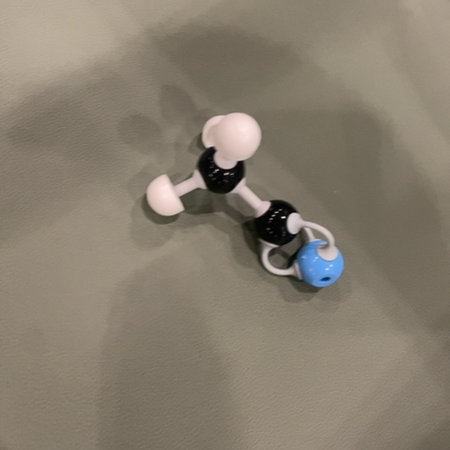
\includegraphics[width=0.15\linewidth]{6342.png} & CC\#N\\ \hline
        Chlorocyclobutane&  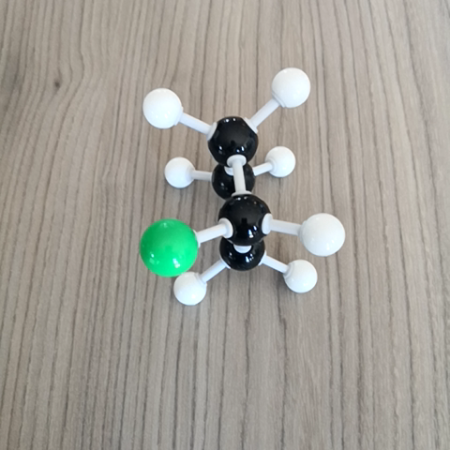
\includegraphics[width=0.15\linewidth]{70712.png} & C1CC(C1)Cl\\ \hline
        2-Chlorocyclohexanol&  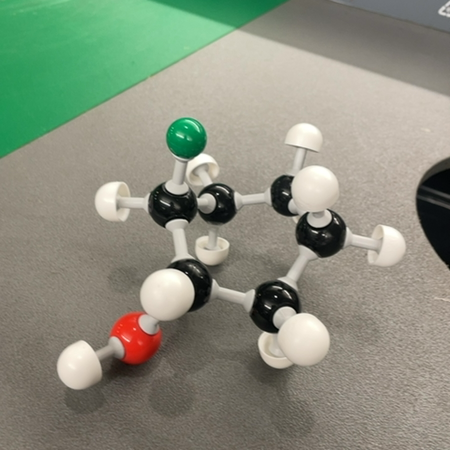
\includegraphics[width=0.15\linewidth]{15274.png} & C1CCC(C(C1)O)Cl\\ \hline
        2,2,3,3-Tetramethylbutane&  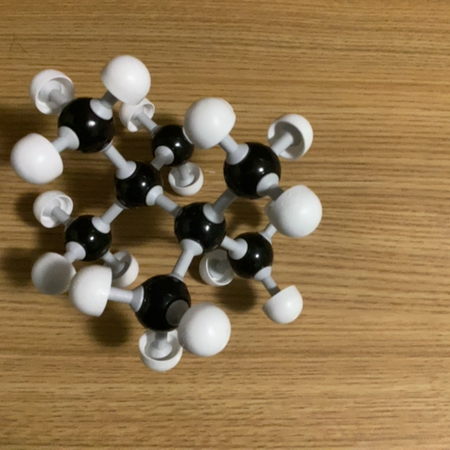
\includegraphics[width=0.15\linewidth]{11675.png} & CC(C)(C)C(C)(C)C\\ \hline
        Deuteriomethane&  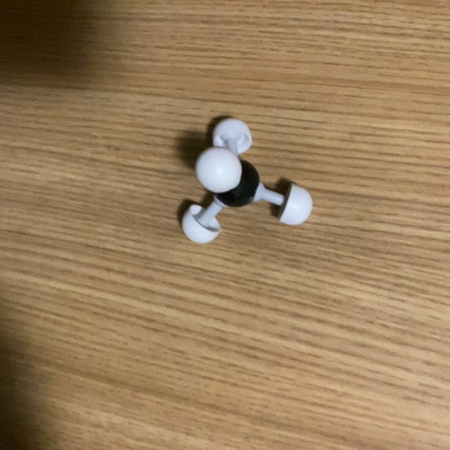
\includegraphics[width=0.15\linewidth]{12669.png} & C\\ \hline
        N-Propyl Isocyanide&  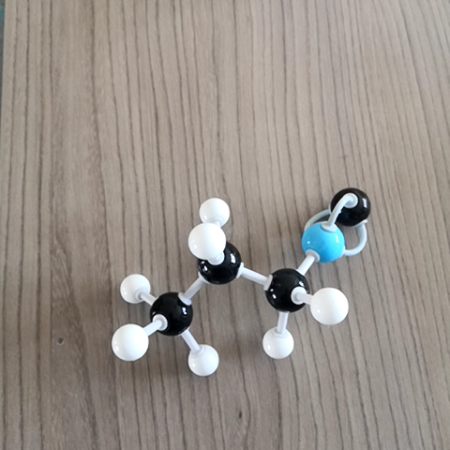
\includegraphics[width=0.15\linewidth]{79084.png} & CCC[N+]\#[C-]\\ \hline
\end{tabular}
\end{center}
\subsection*{Screenshots of the image collecting application}

\begin{center}
    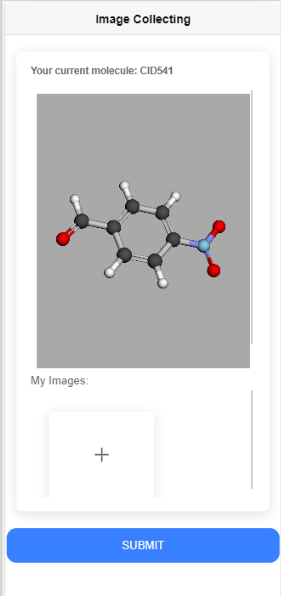
\includegraphics[width=0.3\linewidth]{ss2.png}
    % 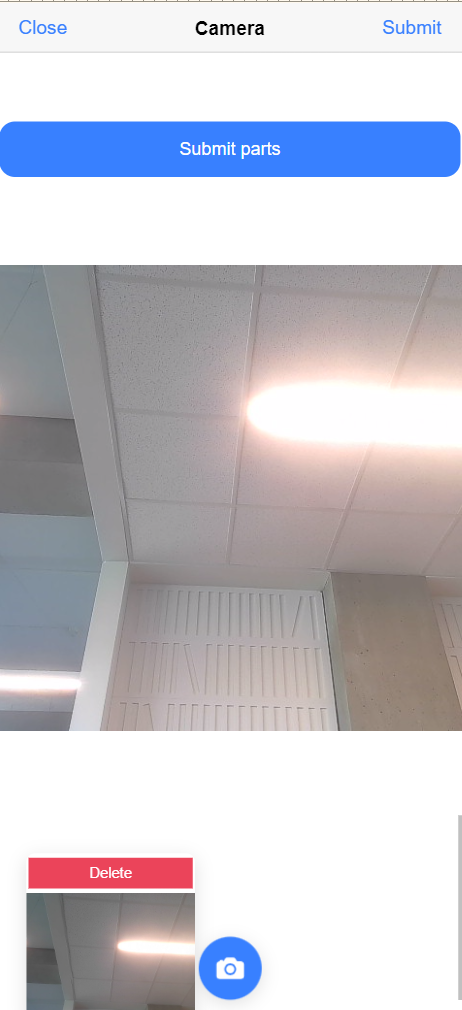
\includegraphics[width=0.25\linewidth]{ss3.png}
\end{center}


\end{document}
